\documentclass[11pt,a4paper]{article}
\usepackage[T1]{fontenc}
\usepackage{lmodern}
\usepackage[margin=2.2cm]{geometry}
\usepackage{amsmath,amssymb,graphicx,booktabs,tabularx,array,float,caption,xcolor}
\usepackage[section]{placeins}
\usepackage{longtable}
\usepackage[numbers,sort&compress]{natbib}
\usepackage[colorlinks=true,linkcolor=blue!45!black,citecolor=blue!45!black,urlcolor=blue!45!black]{hyperref}
\graphicspath{{figures/}}
\captionsetup{font=small,labelfont=bf}
\setlength{\parskip}{3pt}
\makeatletter
\setlength{\@fptop}{0pt}
\setlength{\@fpsep}{14pt}
\setlength{\@fpbot}{0pt plus 1fil}
\makeatother
\renewcommand{\topfraction}{0.95}
\renewcommand{\bottomfraction}{0.95}
\renewcommand{\textfraction}{0.06}
\renewcommand{\floatpagefraction}{0.80}
\setlength{\textfloatsep}{16pt plus 3pt minus 3pt}
\setlength{\floatsep}{14pt plus 3pt minus 3pt}
\setlength{\emergencystretch}{2em}
\renewcommand{\arraystretch}{1.15}
\newcolumntype{Y}{>{\raggedright\arraybackslash}X}
\title{\textbf{VOLT-KD: Amplitude-Preserving Learning\\for Lightweight Multi-Label ECG Classification}}
\author{}
\date{}
\begin{document}
\maketitle
\vspace{-2em}
\begin{abstract}
Lightweight electrocardiogram (ECG) classification requires preserving diagnostic information within a limited computational budget. Per-record, per-lead standardization removes absolute voltage and alters inter-lead amplitude ratios before signals reach the network. We propose VOLT-KD, an amplitude-preserving framework for lightweight multi-label ECG classification. The framework combines millivolt inputs, multiscale depthwise separable convolutions, and short-sequence modeling with diagnostic subclass supervision and cross-fitted foundation-model soft labels. Teachers and auxiliary heads are used only during training; the deployed student contains 107,189 parameters. In five-seed PTB-XL experiments, millivolt inputs increased the same student's macro ROC-AUC from 0.9106 to 0.9277 and hypertrophy ROC-AUC from 0.8285 to 0.9019. A second compact backbone showed consistent improvements. The complete framework achieved macro ROC-AUC $0.9298\pm0.0012$ and macro F1 $0.7542\pm0.0009$, exceeding published MSCA-Mamba means by 0.0300 and 0.0504, respectively. Adding distillation to subclass supervision increased macro F1 by 0.0043 without enlarging the deployed network. Voltage probes, gain responses, and subclass analyses jointly supported the contribution of input amplitude. Subgroup, perturbation, probability-quality, and literature comparisons further characterized the complete framework. Estimated computation was 30.1 MFLOPs, with single-thread CPU inference latency of 32.5 ms on the evaluated platform. These findings connect diagnostic information preservation, compact representations, and training-time knowledge transfer in an empirically grounded design for lightweight ECG classification.
\end{abstract}
\noindent\textbf{Keywords:} electrocardiogram; multi-label classification; amplitude preservation; lightweight networks; knowledge distillation

\section{Introduction}
Twelve-lead multi-label ECG classification identifies normal ECGs, myocardial infarction, ST/T changes, conduction disturbances, and hypertrophy within the same recording\cite{wagner2020}. Unlike binary detection of a single abnormality, this task must handle coexisting diagnoses, class imbalance, and overlapping diagnostic features. Within a ten-second recording, local waveforms encode morphology, interbeat relationships provide temporal information, and lead voltages and their ratios describe spatial distributions. Resource-constrained devices must convert these signals into useful predictions with limited memory and computation. Lightweight design therefore involves both reducing network size and improving the use of diagnostic information available to a compact model. PTB-XL provides patient-disjoint folds and hierarchical diagnostic labels, establishing a common dataset for investigating this problem\cite{wagner2020}.

Existing studies mainly improve classification through feature extraction and information fusion. MSCA-Mamba\cite{cetintas2026}, for example, first standardizes each lead within each recording and then extracts local morphology using multiscale convolutions. Channel recalibration and a state-space module integrate these features before the network outputs multiple diagnostic probabilities. With 121,149 parameters, it achieves macro ROC-AUC 0.8998, demonstrating the feasibility of compact networks for this task. Chimera\cite{behrouz2024} models dynamic temporal and variable dependencies with state-space structures, whereas MS-LTCAF\cite{feng2025} selects informative locations through lead--temporal co-attention. DBA-ASFNet\cite{luo2025} combines depthwise separable residual convolutions, a bidirectional gated recurrent unit (GRU), and demographic information to reduce representation costs. CNN--FFT\cite{malik2026} combines time-domain morphology with frequency-domain features. These approaches offer different solutions for extracting information inside the network. The relationship between amplitude processing before the network and subsequent class-specific gains remains less explicit. When preprocessing maps waveforms to a common scale, does it remove nuisance variation or diagnostic information that the model should retain?

This distinction is directly relevant to hypertrophy recognition, where Sokolow--Lyon and Cornell voltage criteria depend on amplitudes in specific leads\cite{sokolow1949,casale1985,hancock2009}. Per-record, per-lead z-score normalization gives similarly shaped waveforms nearly identical representations despite different absolute amplitudes, while also changing inter-lead amplitude ratios. A network can still exploit morphology and label co-occurrence, but physical voltage no longer enters learning in its original form. Recent DeepECG research also incorporates amplitude handling into foundation-model preprocessing\cite{nolin2026}. We examine how much millivolt-scale preservation benefits a classifier with approximately one hundred thousand parameters, which classes benefit, and whether gains extend across backbones. Controlled comparisons can thus turn preprocessing from a fixed default into a task-informed design decision.

A complementary research direction enriches the knowledge available during training. ECGFounder\cite{li2025} learns diagnostic representations from over ten million recordings, and ECG-FM\cite{mckeen2025} provides an open self-supervised foundation model. MVKT-ECG\cite{qin2023} transfers information from multi-lead teachers to single-lead students through multi-view knowledge transfer. These studies expand the supervision available to small models. However, the relationship among overall teacher performance, class-specific teacher competence, and student input representations warrants targeted evaluation. High aggregate teacher performance does not guarantee equally useful targets for every diagnostic class. PTB-XL also provides twenty-three diagnostic subclasses and higher-rate recordings, offering richer training information than five superclass labels alone. Our second design question concerns how to organize this information for lightweight inference while distinguishing input preservation from additional supervision.

We propose VOLT-KD, an amplitude-preserving framework that integrates physical inputs, compact representations, and training-time knowledge learning into a single classification pipeline. Recordings are converted to millivolts, and only constant lead offsets are removed so that voltage differences enter feature extraction directly. Multiscale depthwise separable convolutions and downsampling extract waveform patterns, while a bidirectional GRU aggregates context over a shortened sequence. Training combines superclass labels, subclass labels, and foundation-model soft labels. Cross-fitting generates each training record's soft targets using a teacher that excluded its fine-tuning fold. Diagnostic subclasses and the higher-rate teacher are restricted to training; deployment retains only the 100 Hz input, student backbone, and five-class prediction head. The framework uses established convolutional, recurrent, and distillation components. Its contribution centers on task-informed amplitude preservation and experimentally testable relationships among input information, supervision, and computational cost.

VOLT-KD has three connected properties that motivate the experimental evaluation. First, information preservation acts at the start of learning. Changing only input processing for the same student increases macro ROC-AUC from 0.9106 to 0.9277 and HYP ROC-AUC from 0.8285 to 0.9019. Second, the compact backbone limits inference cost to 107,189 deployed parameters and an estimated 30.1 MFLOPs. The complete configuration achieves macro ROC-AUC 0.9298 and macro F1 0.7542. Third, fixed-student comparisons identify the contribution of additional supervision, with distillation further improving macro F1 beyond subclass supervision. Evaluation includes recent literature, common-protocol comparisons, diagnostic subclasses, demographic subgroups, probability quality, synthetic perturbations, and inference efficiency. Together, these analyses establish overall performance, identify the sources of gains, and characterize diagnostic coverage and resource requirements.

The main contributions of this study are as follows:
\begin{enumerate}
\item We develop an amplitude-preserving learning pipeline that combines millivolt inputs with multiscale temporal representations for compact multi-label ECG classification. Training-free voltage probes, input controls in two backbones, and gain-response experiments link preserved information to model behavior and hypertrophy-related gains.
\item We organize diagnostic subclasses and cross-fitted teacher probabilities into hierarchical supervision while retaining a single lightweight prediction path at deployment. Additive and removal ablations quantify the dominant input contribution and identify the incremental macro-F1 benefit and class-specific effects of teacher soft labels.
\item We show that a single student with approximately one hundred thousand parameters achieves strong multi-label classification performance on PTB-XL with low computation and high batch throughput. Subclass, test-subgroup, perturbation, and reduced-lead analyses characterize performance and resource trade-offs under different observation conditions.
\end{enumerate}

VOLT-KD combines diagnostic information preservation, compact feature extraction, and training-time knowledge learning so that limited inference capacity can use physical voltage and hierarchical supervision.
\section{Related Work}
\subsection{Compact Networks and Multi-Label Dependencies}
Compact ECG classification requires efficient modeling of local morphology, long-range rhythm, and inter-lead relationships. MSCA-Mamba, published by Cetintas in 2026, combines multiscale convolutions, squeeze-and-excitation attention, and a unidirectional state-space module with approximately 120,000 parameters\cite{cetintas2026}. Chimera models temporal and variable relationships using two-dimensional state-space structures\cite{behrouz2024}, whereas the 2025 MS-LTCAF framework jointly weights lead and temporal positions\cite{feng2025}. ECG-Mamba, also published in 2025, adapts vision Mamba to twelve-lead signals and introduces Non-Uniform-Mix augmentation\cite{jiang2025}. These approaches improve representations through feature aggregation, long-range modeling, and variation in training examples.

Other methods incorporate additional information or label dependencies. DBA-ASFNet combines depthwise separable convolutions, a bidirectional GRU, and demographic information\cite{luo2025}, while CNN--FFT complements temporal features with a deterministic frequency-domain branch\cite{malik2026}. MAR-GCNet, published in 2026, integrates multiscale attention features with graph convolutions over labels to model co-occurring abnormalities\cite{luomar2026}. Label relationships can also inform representation learning through training targets. VOLT-KD jointly learns diagnostic superclasses and subclasses, using finer diagnostic labels during training while retaining five superclass outputs at deployment. We construct the student from established compact components and test physical voltage information through input comparisons with a fixed backbone. This design allows the effects of computational structure and retained input information to be evaluated separately.

\subsection{Foundation Models and Self-Supervised ECG Representations}
Self-supervised learning provides a route to ECG classification using unlabeled signals. Mehari and Strodthoff investigated label efficiency and noise robustness in twelve-lead self-supervised learning\cite{mehari2022}, while HeartBEiT uses image-based ECG pretraining for downstream diagnosis\cite{vaid2023}. ECGFounder, published in 2025, applies supervised pretraining to over ten million recordings\cite{li2025}. ECG-FM combines masked reconstruction, contrastive learning, and ECG-specific augmentation in an open foundation model\cite{mckeen2025}. ECG-JEPA instead predicts latent features of masked segments, learning representations from ten public databases and offering an alternative to signal reconstruction or objectives based on handcrafted augmentations\cite{weimann2025}.

Research in 2026 further examines task coverage and pretraining data. ECG-LFM combines contextual contrastive learning, masked modeling, and multi-segment contrastive learning for cardiovascular disease prediction and genetic association analysis\cite{lin2026}. DeepECG evaluates supervised and self-supervised foundation models across multiple tasks, external datasets, and computational requirements\cite{nolin2026}. Khattak et al. show that pretraining data composition affects the performance and generalizability of contrastive ECG foundation models\cite{khattak2026}. Together, these studies indicate that the value of teacher knowledge depends on learning objectives, training data, and downstream tasks. VOLT-KD converts an existing ECGFounder model's knowledge into training-time probability targets, allowing a compact 100 Hz student to use diagnostic information from a 500 Hz teacher. Comparisons of supervision components then assess the resulting student-level benefits.

\subsection{Knowledge Distillation and Diagnostic Supervision}
Knowledge distillation guides a student using teacher outputs or intermediate representations to reduce deployment cost. MVKT-ECG combines multi-view knowledge transfer and multi-label distillation to transfer multi-lead information to a single-lead student\cite{qin2023}. HMT-KD, published in 2026, introduces a teacher assistant between two primary teachers and the final student, combining response-based and feature-based distillation\cite{beigzadeh2026}. SKD-AMBRNet, also published in 2026, constructs an auxiliary self-teacher from residual branches at different student depths and strengthens supervision with spatial and channel attention\cite{qian2026}. MDOT incorporates physician-defined features, including heart rate, QRS duration, ST changes, and QTc, into a teacher and uses momentum distillation to train its student\cite{yisimitila2025}. These approaches organize supervision around teacher hierarchies, internal network knowledge, and clinical priors, respectively.

VOLT-KD integrates supervision design with amplitude preservation. Five diagnostic superclasses define the target task, twenty-three subclasses supply finer labels, and cross-fitted teacher probabilities provide soft supervision. The teacher and subclass head are used during training, with a single compact student retained for inference. We investigate how these information sources complement one another within the same student, comparing input representations, subclass supervision, and distillation configurations and examining class-specific responses. The comparative preprint released by Mert et al. in September 2026 evaluates 1D-ResNet18, bidirectional Mamba, xLSTM, CWT-ViT-KAN, fine-tuned ECGFounder, and heterogeneous ensembles on the same five-class task\cite{mert2026}. It provides a recent reference for positioning lightweight single-model performance across inference configurations.

\subsection{Amplitude Information, Signal Quality, and Lead Availability}
Physical ECG amplitude reflects acquisition conditions while carrying diagnostically relevant information. DeepECG includes amplitude-range handling in preprocessing across data sources\cite{nolin2026}, providing a recent context for amplitude preservation. VOLT-KD compares per-record, per-lead z-score normalization with millivolt inputs under controlled conditions. Voltage probes, two compact backbones, and gain interventions connect changes in input representation to classification performance and model responses. The central question is which information retained before inference can be used by a compact network, and how its benefit is distributed across diagnostic classes.

Missing leads and signal corruption change the observations available for classification. TolerantECG, published in 2025, combines contrastive learning between ECGs and knowledge-retrieval-enhanced reports with self-supervised learning on corrupted or lead-missing signals, supporting arbitrary lead subsets and noisy inputs\cite{nguyen2025}. In 2026, Su et al. proposed cross-lead distillation from a twelve-lead teacher to a lightweight single-lead student for normal--abnormal screening\cite{su2026}. These studies emphasize incomplete-signal representations and cross-lead deployment, respectively. We use twelve-lead, five-superclass classification as the primary task and additionally evaluate separately trained six-limb-lead and lead-II VOLT-KD students, together with the complete model under test-time noise and random lead loss. These evaluations connect input information preservation, training-time knowledge transfer, and changes in acquisition conditions within one framework.

\section{Method}
\subsection{Task Definition and Framework}
For a ten-second twelve-lead recording sampled at 100 Hz, the student receives $X\in\mathbb R^{12\times1000}$ and outputs five independent diagnostic probabilities $p\in[0,1]^5$. The binary label vector $y\in\{0,1\}^5$ allows co-occurrence among normal ECG (NORM), myocardial infarction (MI), ST/T changes (STTC), conduction disturbance (CD), and hypertrophy (HYP). Training additionally uses twenty-three diagnostic subclass labels $u\in\{0,1\}^{23}$.

VOLT-KD combines amplitude-preserving preprocessing, a lightweight student backbone, and hierarchical supervision during training (Figure~\ref{fig:framework}). Millivolt inputs preserve waveform voltage, and multiscale convolution with short-sequence modeling extracts compact features. Superclass labels, subclass labels, and ECGFounder teacher probabilities jointly supervise training. At inference, the teacher and auxiliary subclass head are removed, retaining only the student backbone and five-class prediction head.
\begin{figure}[htbp]
\centering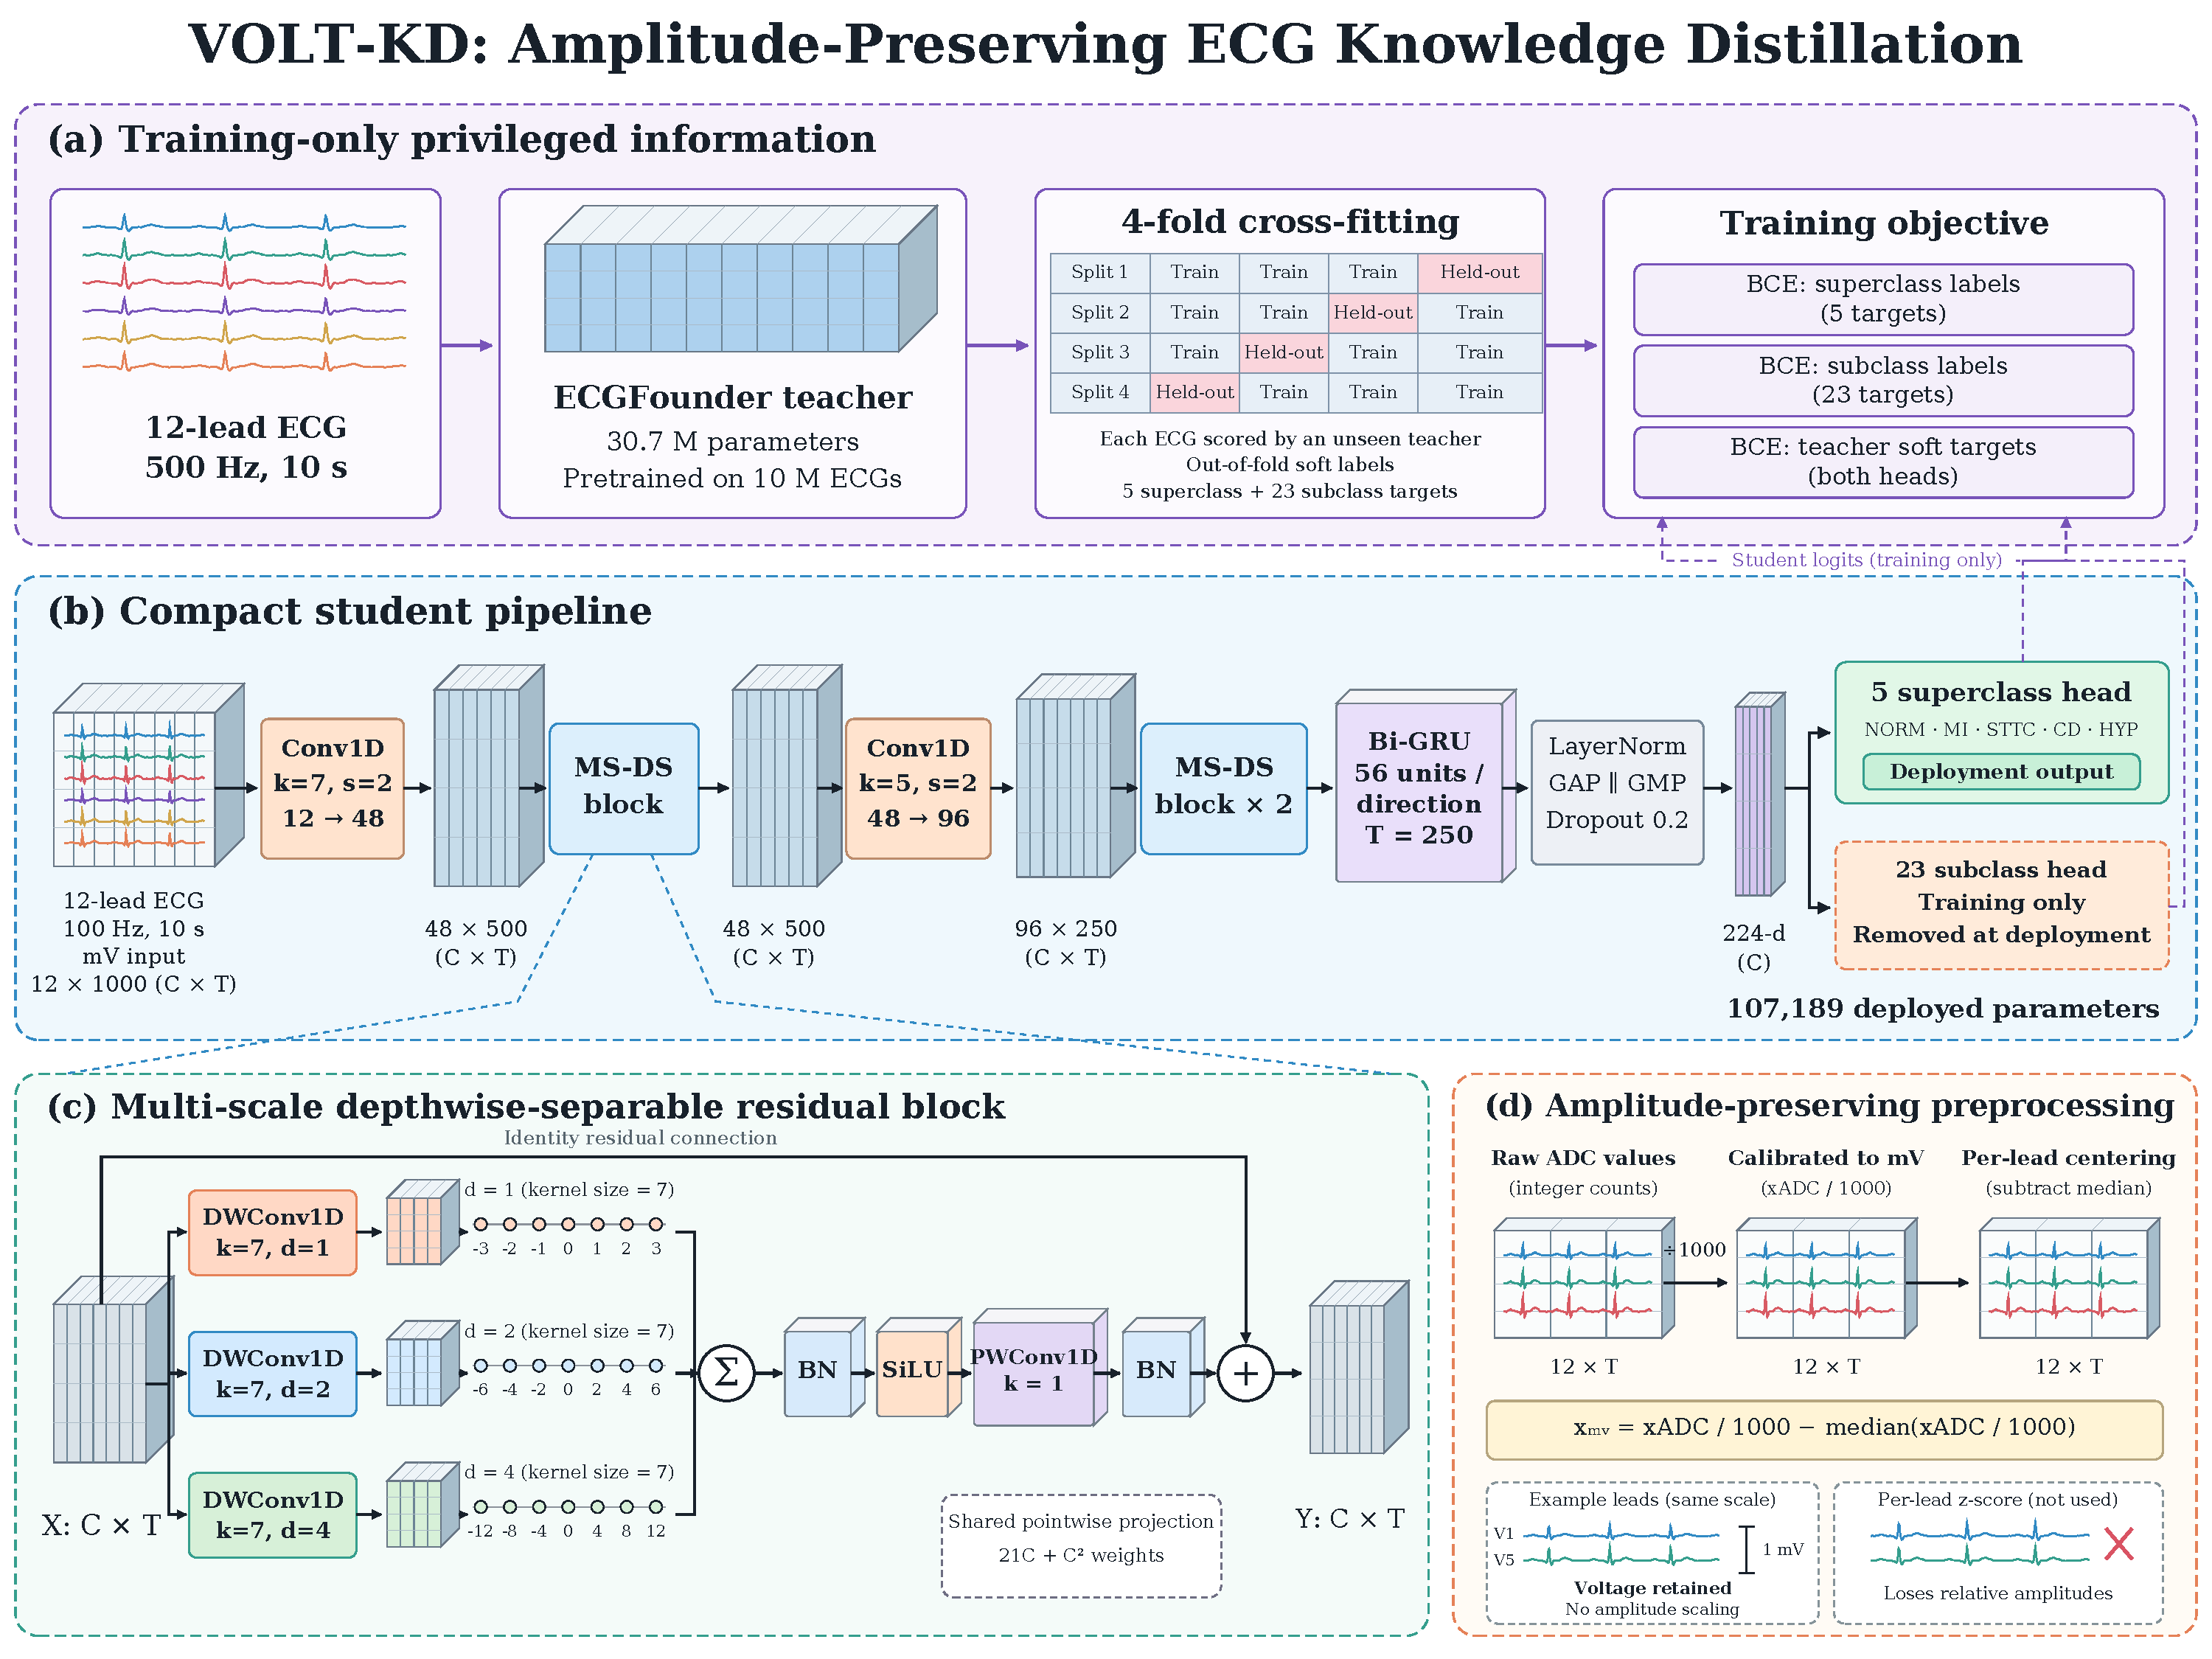
\includegraphics[width=\linewidth]{f02_architecture.pdf}
\caption{Overview of VOLT-KD. (a) A 500 Hz ECGFounder teacher provides cross-fitted soft labels for superclass and subclass supervision. (b) The compact student processes 100 Hz millivolt inputs and retains only the five-superclass head at deployment, with 107,189 parameters. (c) The multiscale depthwise-separable residual block uses dilation rates 1, 2, and 4 with a shared pointwise projection. (d) ADC-to-millivolt calibration and per-lead median centering preserve voltage amplitude. GAP and GMP denote global average and maximum pooling.}
\label{fig:framework}
\end{figure}

\subsection{Preserving Physical Amplitude}
Amplitude processing distinguishes constant offsets from the voltage carried by a waveform. For lead $\ell$ of a single recording, per-lead standardization is defined as
\begin{equation}
 Z_\ell(X)=\frac{X_\ell-\mu_\ell}{s_\ell+\epsilon},
\end{equation}
where $\mu_\ell$ and $s_\ell$ are computed from that recording and $\epsilon=10^{-6}$. Neglecting the stabilizing term and assuming $s_\ell>0$, a positive gain $a_\ell$ and constant offset $b_\ell$ satisfy
\begin{equation}
 Z_\ell(a_\ell X_\ell+b_\ell)=Z_\ell(X_\ell).
\end{equation}
Thus, identically shaped signals with different absolute amplitudes map to the same representation. Standardization aligns input scales while removing the scale itself from subsequent learning.

To retain this information, we convert analog-to-digital converter (ADC) values to millivolts using the stored gain and subtract each lead's temporal median:
\begin{equation}
 \widetilde X_\ell(t)=X^{\mathrm{ADC}}_\ell(t)/1000
 -\operatorname{median}_{\tau}\big(X^{\mathrm{ADC}}_\ell(\tau)/1000\big).
\end{equation}
The constant 1000 is the ADC gain of the PTB-XL data used here. This operation removes constant offsets while preserving waveform amplitudes in millivolts. The network then processes voltage differences across leads and recordings. No per-record scale division is applied, and preprocessing is identical during training and inference.

\subsection{Compact Multiscale Temporal Representations}
ECG structures with different durations require different temporal receptive fields. Three depthwise branches with dilation rates 1, 2, and 4 extract multiscale features, with a shared pointwise projection limiting channel-mixing costs\cite{howard2017}. Each branch uses a kernel of 7. Their summed outputs pass through batch normalization, a sigmoid linear unit (SiLU), pointwise convolution, and batch normalization, followed by a residual connection. For $C$ channels, the weight count is $21C+C^2$, excluding biases and normalization parameters, compared with $21C^2$ for three full-convolution branches. Separating temporal-scale expansion from channel mixing therefore keeps multiscale extraction compact.

The backbone first maps twelve leads to 48 channels using a kernel-7, stride-2 convolution, followed by one multiscale block. A second kernel-5, stride-2 convolution expands the representation to 96 channels and is followed by two multiscale blocks. The two downsampling steps reduce sequence length from 1000 to 250, shortening subsequent temporal processing. A bidirectional GRU with 56 hidden units per direction aggregates context\cite{cho2014}. Layer-normalized features undergo both global average and global maximum pooling. The concatenated features pass through dropout at rate 0.2 and two independent linear heads predicting five superclasses and twenty-three subclasses.

The training network contains 112,364 parameters, including 5,175 parameters in the subclass head. Removing this head leaves 107,189 parameters at deployment. Auxiliary supervision influences superclass predictions through the shared backbone while preserving a single student inference path.

\subsection{Hierarchical Knowledge Learning During Training}
Five superclass labels define the primary task, and twenty-three subclass labels provide finer diagnostic descriptions. Independent superclass and subclass heads use binary cross-entropy (BCE) for the two levels of supervision. ECGFounder\cite{li2025} is fine-tuned on 500 Hz recordings for the same twenty-eight targets. Its outputs supervise the 100 Hz student, restricting the additional information source to training.

To generate held-out soft labels, training folds 1--8 are divided into four groups of two folds. Each teacher is fine-tuned on six folds and generates logits for the remaining two. The teacher associated with each student training record therefore excludes that patient's fold during fine-tuning. Teacher inputs are standardized using one mean and standard deviation across all time points and leads of each recording, preserving inter-lead amplitude ratios. Each teacher is trained for eight epochs using AdamW, batch size 64, weight decay $10^{-2}$, and a one-cycle schedule peaking at $3\times10^{-4}$. Validation fold 9 selects the checkpoint used for evaluation and soft-label generation.

Let $z^s,z^u$ denote the student's superclass and subclass logits, and let $t^s,t^u$ denote the corresponding teacher logits. The complete training objective is
\begin{align}
 \mathcal L={}&\operatorname{BCE}(z^s,y)+\operatorname{BCE}(z^u,u)\nonumber\\
 &+\operatorname{BCE}(z^s,\sigma(t^s))+\operatorname{BCE}(z^u,\sigma(t^u)).
\end{align}
The first two terms align student predictions with diagnostic labels, and the last two provide soft supervision from teacher probabilities\cite{hinton2015}. BCE is implemented directly on logits. Each term is averaged over batch samples and the classes of its corresponding head, with unit weights and temperature 1. The two heads predict independently, while subclass supervision shapes their shared features. Cross-fitting ensures that soft labels satisfy the patient-fold exclusion constraint during teacher fine-tuning.

\subsection{Voltage Probes and Model-Response Analysis}
We evaluate input information and model behavior at two complementary levels. Training-free voltage probes measure the discrimination of voltage statistics before and after preprocessing. Gain perturbations then test whether trained models respond to changes in amplitude.

The probes follow Sokolow--Lyon and Cornell forms\cite{sokolow1949,casale1985}. For centered recordings, the 99th percentile approximates R-wave amplitude $R_\ell$, and the negative first percentile approximates S-wave depth $S_\ell$. We compute
\begin{equation}
 V_{\mathrm{SL}}=S_{V1}+\max(R_{V5},R_{V6}),\qquad
 V_{\mathrm C}=R_{aVL}+S_{V3}.
\end{equation}
These statistics are evaluated on millivolt and standardized inputs using ROC-AUC for the left ventricular hypertrophy (LVH) subclass and HYP superclass. Percentiles are computed over each complete ten-second recording, and positive targets are ECG interpretation labels in the database. Gain experiments multiply test waveforms by specified factors while fixing labels, model weights, and validation-derived thresholds. Changes in predicted probabilities and positive-call rates quantify the resulting responses.

\section{Experiments and Results}
\subsection{Data and Experimental Setup}
We used PTB-XL 1.0.3\cite{wagner2020}, containing 21,799 recordings from 18,869 patients. After excluding 411 recordings without diagnostic labels, official patient-disjoint folds 1--8, 9, and 10 defined training, validation, and test sets, respectively. These sets contained 17,084, 2,146, and 2,158 recordings. Table~\ref{tab:data} summarizes class distributions across the three partitions. All five diagnostic superclasses were included, with label co-occurrence handled through the multi-label objective.
\begin{table}[htbp]
\centering\small
\caption{Diagnostic-task partitions of PTB-XL 1.0.3. Parentheses indicate the percentage of positive recordings; diagnostic labels can co-occur.}\label{tab:data}
\begin{tabularx}{\linewidth}{Yrrr}
\toprule
Class & Training & Validation & Test \\
\midrule
NORM & 7596 (44.46\%) & 955 (44.50\%) & 963 (44.62\%) \\
MI & 4379 (25.63\%) & 540 (25.16\%) & 550 (25.49\%) \\
STTC & 4186 (24.50\%) & 528 (24.60\%) & 521 (24.14\%) \\
CD & 3907 (22.87\%) & 495 (23.07\%) & 496 (22.98\%) \\
HYP & 2119 (12.40\%) & 268 (12.49\%) & 262 (12.14\%) \\
Records & 17,084 & 2,146 & 2,158 \\
\bottomrule
\end{tabularx}

\end{table}

Students were trained for twenty-four epochs using AdamW\cite{loshchilov2019}, batch size 64, and weight decay $10^{-2}$. A one-cycle schedule peaked at $4\times10^{-3}$, with the increasing phase occupying 15\% of training steps and gradient norms capped at 2. Augmentation comprised random circular shifts, per-record gains of 0.9--1.1, and Gaussian noise with standard deviation 0.01 in the corresponding input units. Evaluation used exponential moving-average weights with nominal decay 0.999, updated every four steps with an initial correction. Validation macro ROC-AUC selected checkpoints. Class-specific thresholds maximized validation F1 over a 0.05--0.95 grid with step 0.01.

Main experiments used seeds 42, 123, 456, 789, and 2025, with results reported as mean and sample standard deviation. Macro ROC-AUC measures classwise ranking, macro average precision (AP) measures precision--recall performance, and macro F1 evaluates decisions at fixed thresholds. AP follows the average-precision definition. Intervals in Table~\ref{tab:effects} use paired metric differences for identical seeds and describe training variability on the fixed test set. The comparisons are reported as exploratory effect estimates.

VOLT-KD input and supervision controls fixed the student backbone, data splits, and training recipe; structural ablations changed only the specified modules. Superclass-only training used five hard labels, superclass-plus-subclass training added subclass targets, and complete supervision further incorporated ECGFounder soft labels. Cross-backbone input experiments used a local MSCA-Mamba implementation with batch size 16, learning rate and weight decay $10^{-4}$, and at most thirty epochs. Early stopping used a patience of seven epochs. Millivolt inputs were median-centered, whereas z-score inputs were mean-centered and scaled by their standard deviations. Student noise augmentation was applied in each representation's own units, so input comparisons evaluated each preprocessing-and-augmentation combination. The main comparison used published MSCA-Mamba results. Input controls, perturbations, subgroup analyses, and efficiency measurements used predictions and measurements from the local implementation.
\subsection{Overall Comparison with Existing Methods}
VOLT-KD improved both multi-label ranking and classification decisions with approximately one hundred thousand deployed parameters (Table~\ref{tab:main}). Macro ROC-AUC was $0.9298\pm0.0012$, compared with the published MSCA-Mamba result of $0.8998\pm0.0022$. Macro PR-AUC/AP and F1 were 0.8274 and 0.7542, respectively, compared with published values of 0.7651 and 0.7038. Micro-averaged metrics, weighted F1, and subset accuracy also increased. Improvements in macro metrics indicate gains when classes receive equal weight. Higher subset accuracy means that more recordings had all five labels predicted correctly. The complete framework therefore improved both classwise ranking and recording-level multi-label predictions.
\begin{table}[htbp]
\centering\footnotesize
\caption{Full metric comparison with MSCA-Mamba. MSCA-Mamba values are taken directly from Cetintas\cite{cetintas2026}; both methods report means and standard deviations over five seeds. Differences are VOLT-KD minus the published mean; bold denotes the higher result in each row.}\label{tab:main}
\begin{tabularx}{\linewidth}{Yrrr}
\toprule
Metric & \shortstack{MSCA-Mamba\\Published\cite{cetintas2026}} & VOLT-KD & Difference \\
\midrule
Macro ROC-AUC & $0.8998\pm0.0022$ & $\boldsymbol{0.9298\pm0.0012}$ & +0.0300 \\
Micro ROC-AUC & $0.9119\pm0.0052$ & $\boldsymbol{0.9405\pm0.0011}$ & +0.0286 \\
Macro PR-AUC/AP & $0.7651\pm0.0036$ & $\boldsymbol{0.8274\pm0.0020}$ & +0.0623 \\
Macro F1 & $0.7038\pm0.0045$ & $\boldsymbol{0.7542\pm0.0009}$ & +0.0504 \\
Micro F1 & $0.7474\pm0.0074$ & $\boldsymbol{0.7882\pm0.0021}$ & +0.0408 \\
Weighted F1 & $0.7494\pm0.0039$ & $\boldsymbol{0.7867\pm0.0007}$ & +0.0373 \\
Subset accuracy & $0.5691\pm0.0143$ & $\boldsymbol{0.6168\pm0.0131}$ & +0.0477 \\
\bottomrule
\end{tabularx}
\par\vspace{3pt}{\footnotesize PR-AUC and AP retain the terminology of their respective sources; this study computes average precision. Published means are used for descriptive comparison.}
\end{table}



Recent literature further places VOLT-KD within the trade-off between accuracy and model size (Table~\ref{tab:recent} and Supplementary Table~S9). Its macro ROC-AUC, PR-AUC/AP, and F1 exceeded the ResNet18, bidirectional Mamba, xLSTM, and CWT-ViT-KAN results reported by Mert et al. Broader references showed different strengths: CNN--FFT reported macro F1 0.770, whereas DBA-ASFNet achieved AUC 0.9166 with approximately 0.030 million parameters. Chimera and fine-tuned ECGFounder reported AUC 0.930, and heterogeneous stacking reached 0.936. A single compact 100 Hz VOLT-KD student approached the ranking performance of some higher-capacity or higher-rate methods while confining rich supervision to training. Literature protocols differ in inputs, pretraining resources, and evaluation. These comparisons characterize the trade-off between resources and performance, while local controlled experiments assess individual component contributions.
\begin{table}[htbp]
\centering\footnotesize
\caption{Author-reported results from 2025--2026 on PTB-XL's five diagnostic superclasses. Sources: Cetintas (2026)\cite{cetintas2026}, Mert et al. (2026 preprint)\cite{mert2026}, and Feng et al. (2025)\cite{feng2025}. VOLT-KD results are from this study; parameter counts are in millions (M).}\label{tab:recent}
\begin{tabularx}{\linewidth}{Yc p{1.65cm} rrrr}
\toprule
Method and source & Year & Input & Parameters & \shortstack{Macro\\ROC-AUC} & \shortstack{PR-AUC\\/AP} & \shortstack{Macro\\F1} \\
\midrule
MSCA-Mamba\cite{cetintas2026} & 2026 & 100 Hz & 0.1211 & $0.8998\pm0.0022$ & 0.7651 & 0.7038 \\
1D-ResNet18\cite{mert2026} & 2026 & 100 Hz & -- & 0.922 & 0.797 & 0.738 \\
Bidirectional Mamba\cite{mert2026} & 2026 & 100 Hz & -- & 0.923 & 0.816 & 0.739 \\
xLSTM\cite{mert2026} & 2026 & 100 Hz & -- & 0.910 & 0.782 & 0.718 \\
CWT-ViT-KAN\cite{mert2026} & 2026 & 100 Hz & -- & 0.874 & 0.709 & 0.664 \\
MS-LTCAF$^{*}$\cite{feng2025} & 2025 & 100 Hz & 24.585 & 0.927$^{*}$ & -- & 0.745$^{*}$ \\
VOLT-KD (ours) & -- & 100 Hz & \textbf{0.1072} & $\boldsymbol{0.9298\pm0.0012}$ & \textbf{0.8274} & \textbf{0.7542} \\
\bottomrule
\end{tabularx}
\par\vspace{3pt}{\footnotesize Bold marks the best reported value for each metric within this table. $^{*}$ MS-LTCAF reports AUC/F1 without explicitly identifying macro averaging and is included as contextual evidence. The four Mert et al. entries come from one 2026 preprint and use seed 42. Chimera, DBA-ASFNet, CNN--FFT, directly fine-tuned foundation models, and ensembles appear in Supplementary Table~S9. VOLT-KD uses teacher supervision during training and deploys only the student. Dataset versions, inputs, thresholds, and training follow each source's protocol; -- indicates an unreported value in the inspected results.}
\end{table}

VOLT-KD had higher means across all five metrics than the nine compact configurations reported in the MSCA-Mamba paper (Table~\ref{tab:published}). The matched GRU achieved macro AUC 0.9062 and F1 0.7115, below VOLT-KD by 0.0236 and 0.0427, respectively. All 45 configuration--metric comparisons favored VOLT-KD in mean value. The gap persisted across convolutional, recurrent, state-space, and attention variants, indicating room for improvement beyond the choice of network module. This observation is consistent with VOLT-KD's joint emphasis on input information and training supervision.
\begin{table}[htbp]
\centering\footnotesize
\setlength{\tabcolsep}{3pt}
\caption{VOLT-KD versus compact network configurations reported in the MSCA-Mamba paper\cite{cetintas2026}. Values are five-seed means and standard deviations; bold denotes the highest mean in each column.}\label{tab:published}
\begin{tabularx}{\linewidth}{Yrrrrr}
\toprule
Configuration & Macro AUC & PR-AUC/AP & Macro F1 & Micro AUC & Micro F1 \\
\midrule
MSCA-Mamba & $0.8998\pm0.0022$ & $0.7651\pm0.0036$ & $0.7038\pm0.0045$ & $0.9119\pm0.0052$ & $0.7474\pm0.0074$ \\
No SE & $0.8997\pm0.0016$ & $0.7644\pm0.0037$ & $0.7012\pm0.0024$ & $0.9128\pm0.0031$ & $0.7462\pm0.0044$ \\
Multiscale CNN & $0.9012\pm0.0013$ & $0.7644\pm0.0019$ & $0.7010\pm0.0034$ & $0.9175\pm0.0025$ & $0.7492\pm0.0065$ \\
Single scale + SE + Mamba & $0.8964\pm0.0011$ & $0.7579\pm0.0017$ & $0.6977\pm0.0029$ & $0.9140\pm0.0020$ & $0.7438\pm0.0024$ \\
Matched Conv1D & $0.9043\pm0.0014$ & $0.7719\pm0.0027$ & $0.7094\pm0.0055$ & $0.9225\pm0.0018$ & $0.7540\pm0.0075$ \\
Matched GRU & $0.9062\pm0.0014$ & $0.7764\pm0.0026$ & $0.7115\pm0.0036$ & $0.9251\pm0.0010$ & $0.7559\pm0.0024$ \\
Matched LSTM & $0.9044\pm0.0010$ & $0.7706\pm0.0030$ & $0.7070\pm0.0018$ & $0.9227\pm0.0026$ & $0.7524\pm0.0041$ \\
Matched Transformer & $0.8971\pm0.0008$ & $0.7569\pm0.0018$ & $0.7018\pm0.0043$ & $0.9161\pm0.0006$ & $0.7484\pm0.0043$ \\
BiMamba & $0.9047\pm0.0018$ & $0.7712\pm0.0038$ & $0.7098\pm0.0032$ & -- & -- \\
\midrule
VOLT-KD (ours) & $\boldsymbol{0.9298\pm0.0012}$ & $\boldsymbol{0.8274\pm0.0020}$ & $\boldsymbol{0.7542\pm0.0009}$ & $\boldsymbol{0.9405\pm0.0011}$ & $\boldsymbol{0.7882\pm0.0021}$ \\
\bottomrule
\end{tabularx}
\par\vspace{3pt}{\footnotesize Weighted F1 and subset accuracy for complete MSCA-Mamba appear in the main comparison table. Metrics omitted for BiMamba in the source are marked --.}
\end{table}


\subsection{Voltage Probes Establish the Discriminative Value of Amplitude}\label{sec:voltage}
Millivolt representations retained voltage information associated with hypertrophy labels (Figure~\ref{fig:voltage}). On the same test set, the Sokolow--Lyon probe achieved LVH ROC-AUC 0.876 with millivolt inputs and 0.591 after per-lead standardization. Corresponding HYP superclass values were 0.786 and 0.527. Cornell LVH ROC-AUC also decreased from 0.745 to 0.614. Although the two probes combined different lead amplitudes, both lost discrimination after scale normalization. This pattern implicates voltage information rather than a single lead combination.

The voltage probes require no neural-network training, so these differences arise before feature learning. Per-lead z-score normalization changes absolute voltage and inter-lead amplitude ratios, separating the standardized values from the physical quantities on which the probes depend. VOLT-KD removes constant offsets while retaining the millivolt scale, supplying this label-related information directly to a lightweight network without adding parameters. These results support the task-specific motivation for amplitude preservation independently of the backbone and teacher supervision.
\begin{figure}[htbp]
\centering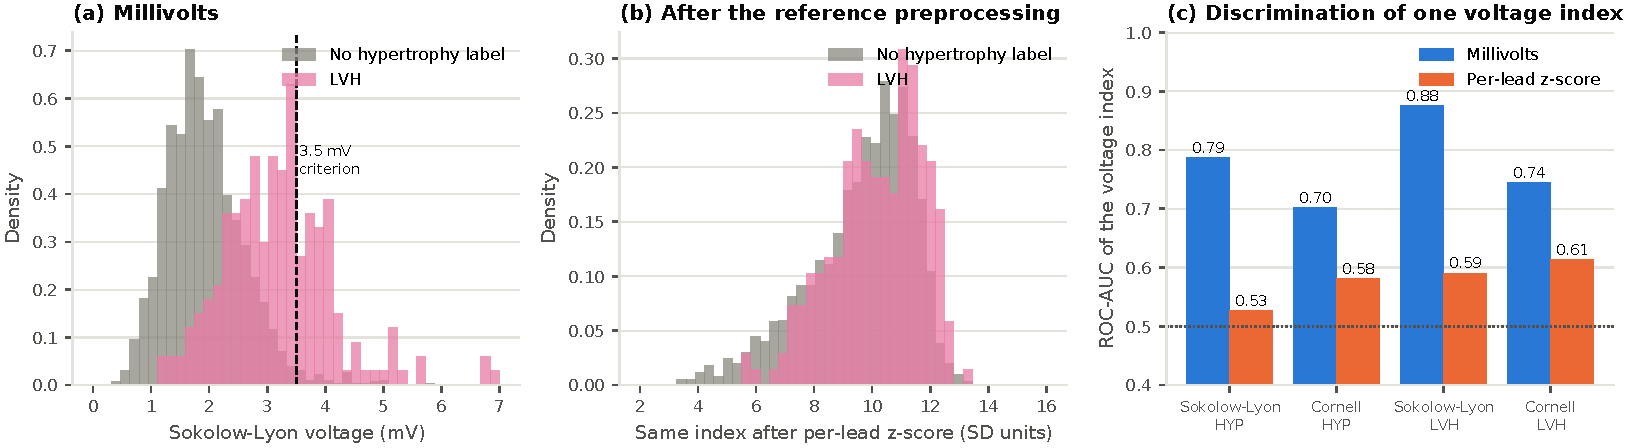
\includegraphics[width=\linewidth]{f03_voltage.pdf}
\caption{Training-free voltage probes. Distributions and discrimination are shown for millivolt and per-lead standardized signals. LVH denotes the left ventricular hypertrophy subclass, and HYP denotes the hypertrophy superclass. Whole-record quantile approximations support information analysis and are not clinical manual measurements.}
\label{fig:voltage}
\end{figure}

\subsection{Contribution of Amplitude Preservation to VOLT-KD}\label{sec:input}
Amplitude preservation produced the main classification gains with a fixed student architecture and remained beneficial under complete supervision (Table~\ref{tab:ladder}). With identical subclass and teacher supervision, millivolt inputs increased macro ROC-AUC from 0.9179 to 0.9298, macro AP from 0.7949 to 0.8274, and macro F1 from 0.7283 to 0.7542. HYP ROC-AUC also increased from 0.8414 to 0.8945. Because capacity and supervision were unchanged, the gains across aggregate metrics and HYP discrimination support voltage preservation as an effective signal representation for knowledge learning.

With only five superclass hard labels, millivolt inputs increased the VOLT-KD student's macro ROC-AUC from 0.9106 to 0.9277. The five-seed paired difference was 0.0171, with a 95\% interval of [0.0142, 0.0201], while macro F1 increased from 0.7189 to 0.7484. HYP ROC-AUC increased by 0.0734, from 0.8285 to 0.9019, accounting arithmetically for approximately 85.7\% of the macro-AUC gain. This concentration agrees with the voltage probes: restoring amplitude-related cues particularly benefits hypertrophy recognition. The benefit was already present before subclass or teacher supervision, establishing input design as a foundational component of the framework.

Input gains under both supervision settings show that amplitude preservation benefits hard-label training and remains compatible with training-time knowledge learning (Figure~\ref{fig:ladder}). Complete VOLT-KD achieved higher macro AUC, AP, and F1, whereas the superclass-only millivolt student achieved higher HYP AUC. Aggregate decision quality and single-class ranking therefore respond differently to supervision. Input and supervision contributions should consequently be evaluated separately.

\begin{table}[htbp]
\centering\footnotesize
\setlength{\tabcolsep}{3pt}
\caption{Input and supervision ablations of the VOLT-KD student. Values are five-seed means and standard deviations. Complete supervision combines superclass hard labels, subclass targets, and ECGFounder soft labels; bold indicates the highest mean per column.}\label{tab:ladder}
\begin{tabularx}{\linewidth}{Yrrrr}
\toprule
Configuration & Macro AUC & HYP AUC & Macro AP & Macro F1 \\
\midrule
VOLT-KD (superclasses only, z-score) & $0.9106\pm0.0008$ & $0.8285\pm0.0044$ & $0.7795\pm0.0019$ & $0.7189\pm0.0039$ \\
VOLT-KD (superclasses only, mV) & $0.9277\pm0.0017$ & $\boldsymbol{0.9019\pm0.0026}$ & $0.8238\pm0.0029$ & $0.7484\pm0.0028$ \\
VOLT-KD (superclasses + subclasses, mV) & $0.9280\pm0.0023$ & $0.9018\pm0.0033$ & $0.8240\pm0.0043$ & $0.7499\pm0.0022$ \\
\midrule
VOLT-KD (complete supervision, z-score) & $0.9179\pm0.0011$ & $0.8414\pm0.0039$ & $0.7949\pm0.0022$ & $0.7283\pm0.0022$ \\
VOLT-KD (complete, mV) & $\boldsymbol{0.9298\pm0.0012}$ & $0.8945\pm0.0018$ & $\boldsymbol{0.8274\pm0.0020}$ & $\boldsymbol{0.7542\pm0.0009}$ \\
\bottomrule
\end{tabularx}
\par\vspace{3pt}{\footnotesize All configurations use the same VOLT-KD backbone. Superclass-only training uses five hard labels; superclass-plus-subclass training adds subclass targets. Neither uses distillation.}
\end{table}
\begin{figure}[htbp]
\centering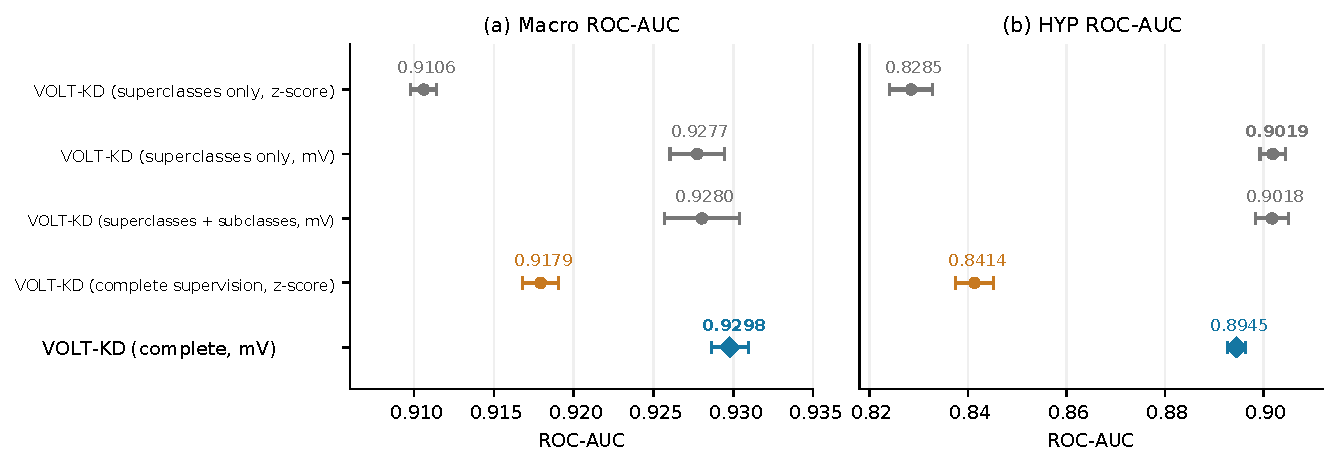
\includegraphics[width=\linewidth]{f11_ablation_ladder.pdf}
\caption{Macro and HYP ROC-AUC for VOLT-KD input and supervision configurations. Blue diamonds denote complete VOLT-KD, orange points its z-score control under complete supervision, and gray points superclass-only or superclass-plus-subclass ablations. Error bars indicate standard deviations over five seeds.}
\label{fig:ladder}
\end{figure}

\subsection{Input-Design Benefits across Backbones}
Amplitude preservation benefited both the recurrent student backbone and the state-space backbone (Table~\ref{tab:backbones}). For the VOLT-KD backbone, macro AUC increased from 0.9106 to 0.9277 under superclass-only supervision and from 0.9179 to 0.9298 under complete supervision. For local MSCA-Mamba, millivolt inputs increased macro AUC from 0.8950 to 0.9157 with the network and training recipe fixed. The paired increase was 0.0207, with a 95\% interval of [0.0188, 0.0227].

Local MSCA-Mamba's HYP ROC-AUC increased from 0.8013 to 0.8879, accounting for approximately 83.5\% of its macro-AUC gain. This classwise pattern resembled that of the VOLT-KD student. Although the backbones aggregate temporal information differently, both benefited primarily in the amplitude-related class. Their agreement supports an input-level benefit that extends beyond a particular sequence module.

The MSCA-Mamba input comparison did not use the VOLT-KD student's noise augmentation, yet showed the same direction of improvement. Together with the complete-supervision input control, these results support amplitude preservation across the two tested compact backbones and different supervision settings. Input design can therefore improve the information available to existing parameters without requiring greater model capacity.

\begin{table}[htbp]
\centering\small
\caption{Input comparisons for VOLT-KD and local MSCA-Mamba. Values are five-seed macro ROC-AUC means and standard deviations. Backbone, supervision, and training settings are fixed within each row; bold indicates the higher result.}\label{tab:backbones}
\begin{tabularx}{\linewidth}{Yrr}
\toprule
Backbone and supervision & z-score Input & mVInput \\
\midrule
VOLT-KD (superclass hard labels) & $0.9106\pm0.0008$ & $\boldsymbol{0.9277\pm0.0017}$ \\
MSCA-Mamba (local) & $0.8950\pm0.0024$ & $\boldsymbol{0.9157\pm0.0012}$ \\
\midrule
VOLT-KD (complete) & $0.9179\pm0.0011$ & $\boldsymbol{0.9298\pm0.0012}$ \\
\bottomrule
\end{tabularx}
\par\vspace{3pt}{\footnotesize Complete VOLT-KD uses superclass hard labels, diagnostic subclass targets, and teacher soft labels. Its two input configurations use identical supervision.}
\end{table}

\subsection{Training-Time Knowledge Improves Classification Decisions}\label{sec:supervision}
Additional supervision on millivolt representations improved classification decisions while preserving the deployed student architecture. Table~\ref{tab:effects} estimates the incremental contributions of subclass targets and ECGFounder supervision using paired differences across identical seeds.

Adding distillation to superclass-plus-subclass training increased the VOLT-KD student's macro F1 from 0.7499 to 0.7542. The paired gain was 0.0043, with a 95\% interval of [0.0022, 0.0064]. Because thresholds were selected on validation data, this gain reflects improved binary-label decisions. The teacher and auxiliary subclass head are removed at deployment. Additional training knowledge therefore translates into a decision benefit within the fixed student network, without adding inference branches.

Paired macro-AUC gains from subclass supervision and distillation were 0.0003 and 0.0017, respectively, with both intervals including zero. Teacher supervision produced a clearer improvement in macro F1. Relative to the larger AUC gains in input controls, these results distinguish two contributions. Amplitude preservation improves the availability of diagnostic information, while soft supervision further adjusts the precision--recall trade-off at validation-selected thresholds. Subclass targets constrain shared representations at finer diagnostic resolution, although their independent ranking benefit was small in this task.

Teacher knowledge had class-specific effects. The four-teacher ECGFounder ensemble achieved macro AUC 0.9323 and HYP AUC 0.8843. The millivolt VOLT-KD student with subclass supervision but no distillation achieved HYP AUC 0.9018, compared with 0.8945 after distillation. The paired change was $-0.0072$, with a 95\% interval of [$-0.0099$, $-0.0045$]. Improved aggregate F1 coexisted with lower HYP ranking performance, indicating that teacher supervision should be assessed against the target class. The student's amplitude-preserving representation already discriminated HYP well. Knowledge transfer should therefore preserve this strength while using the teacher to improve aggregate decisions.

VOLT-KD trained with in-sample teacher targets achieved macro AUC 0.9304, compared with 0.9298 using cross-fitted teachers. Cross-fitting generates each record's soft label with a teacher that excludes its fine-tuning fold, imposing an explicit holdout constraint on target generation. The in-sample scheme achieved a slightly higher macro-AUC score. The two schemes used six and eight fine-tuning folds, respectively, so teacher training-data quantity also affected their accuracy comparison.
\begin{table}[htbp]
\centering\footnotesize
\setlength{\tabcolsep}{4pt}
\caption{Paired comparisons of VOLT-KD student configurations. Each entry is the five-seed mean difference and 95\% interval for the first configuration minus the second. Positive values favor the first configuration. Intervals describe training variability and are not adjusted for multiple comparisons.}\label{tab:effects}
\begin{tabularx}{\linewidth}{Yrrr}
\toprule
VOLT-KD student contrast (first $-$ second) & Macro AUC & HYP AUC & Macro F1 \\
\midrule
VOLT-KD (superclasses only, mV) $-$ VOLT-KD (superclasses only, z-score) & \shortstack{$+0.0171$\\$[0.0142,\,0.0201]$} & \shortstack{$+0.0734$\\$[0.0682,\,0.0786]$} & \shortstack{$+0.0295$\\$[0.0249,\,0.0340]$} \\
VOLT-KD (superclasses + subclasses, mV) $-$ VOLT-KD (superclasses only, mV) & \shortstack{$+0.0003$\\$[-0.0011,\,0.0017]$} & \shortstack{$-0.0002$\\$[-0.0058,\,0.0055]$} & \shortstack{$+0.0016$\\$[-0.0014,\,0.0045]$} \\
VOLT-KD (complete) $-$ VOLT-KD (superclasses + subclasses, no KD) & \shortstack{$+0.0017$\\$[-0.0003,\,0.0038]$} & \shortstack{$-0.0072$\\$[-0.0099,\,-0.0045]$} & \shortstack{$+0.0043$\\$[0.0022,\,0.0064]$} \\
VOLT-KD (cross-fitted teachers) $-$ VOLT-KD (in-sample teacher) & \shortstack{$-0.0006$\\$[-0.0012,\,-0.0001]$} & \shortstack{$-0.0056$\\$[-0.0080,\,-0.0031]$} & \shortstack{$-0.0018$\\$[-0.0079,\,0.0043]$} \\
\bottomrule
\end{tabularx}
\par\vspace{3pt}{\footnotesize All configurations use millivolt inputs except the input-processing control. The no-distillation student uses superclass and subclass targets. Teacher-scheme comparisons evaluate VOLT-KD students trained using the respective soft labels.}

\end{table}


Training-time knowledge learning connects high-capacity teachers to a low-capacity deployment model (Table~\ref{tab:teacher} and Figure~\ref{fig:teacher}). A single ECGFounder teacher contains 30,693,964 parameters, and the four-teacher ensemble contains 122,775,856 in total. The deployed VOLT-KD student has 107,189 parameters, approximately $1/286.4$ and $1/1145.4$ of these counts, corresponding to reductions of 99.65\% and 99.91\%. Teacher capacity is thereby separated from deployment capacity, allowing additional knowledge to be used without retaining a large inference network.

At this size, VOLT-KD trailed the four-teacher ensemble by only 0.0025 in macro AUC and 0.0031 in AP. Macro F1 increased from the ensemble's 0.7482 to 0.7542, and HYP AUC increased from 0.8843 to 0.8945. Relative to the single eight-fold teacher, student macro AUC was only 0.0005 lower, while AP and F1 were higher by 0.0025 and 0.0086. The small student thus retained near-teacher aggregate ranking performance with higher threshold-based F1. The no-distillation student already achieved high AUC. This performance--size trade-off therefore reflects the combined input, representation, and supervision design, with distillation's measurable increment concentrated in final classification decisions.

\begin{table}[htbp]
\centering\footnotesize
\setlength{\tabcolsep}{3pt}
\caption{Performance and size of ECGFounder teachers and VOLT-KD students. ECGFounder\cite{li2025} results come from project fine-tuning evaluations; teacher results represent one evaluation per configuration, whereas student values are five-seed means. Parameters follow deployment configurations and are expressed in millions (M). Higher performance and lower parameter counts are preferable; best values are bold.}\label{tab:teacher}
\begin{tabularx}{\linewidth}{Ycrrrrr}
\toprule
Configuration & Input & \shortstack{Parameters\\ (M)} & \shortstack{Macro\\AUC} & \shortstack{Macro\\AP} & \shortstack{Macro\\F1} & HYP AUC \\
\midrule
ECGFounder, four-teacher ensemble & 500 Hz & 122.7759 & \textbf{0.9323} & \textbf{0.8305} & 0.7482 & 0.8843 \\
ECGFounder, eight-fold teacher & 500 Hz & 30.6940 & 0.9303 & 0.8249 & 0.7456 & 0.8795 \\
VOLT-KD (no distillation) & 100 Hz & \textbf{0.1072} & $0.9280\pm0.0023$ & 0.8240 & 0.7499 & \textbf{0.9018} \\
VOLT-KD (in-sample teacher) & 100 Hz & \textbf{0.1072} & $0.9304\pm0.0011$ & 0.8282 & \textbf{0.7560} & 0.9001 \\
VOLT-KD & 100 Hz & \textbf{0.1072} & $0.9298\pm0.0012$ & 0.8274 & 0.7542 & 0.8945 \\
\bottomrule
\end{tabularx}
\par\vspace{3pt}{\footnotesize Ensemble parameters sum four independent teachers; test predictions use their averaged logits. Training soft labels come from each record's corresponding held-out teacher. All students share the same deployed architecture without auxiliary heads. Size ratios use unrounded parameter counts.}
\end{table}

\begin{figure}[htbp]
\centering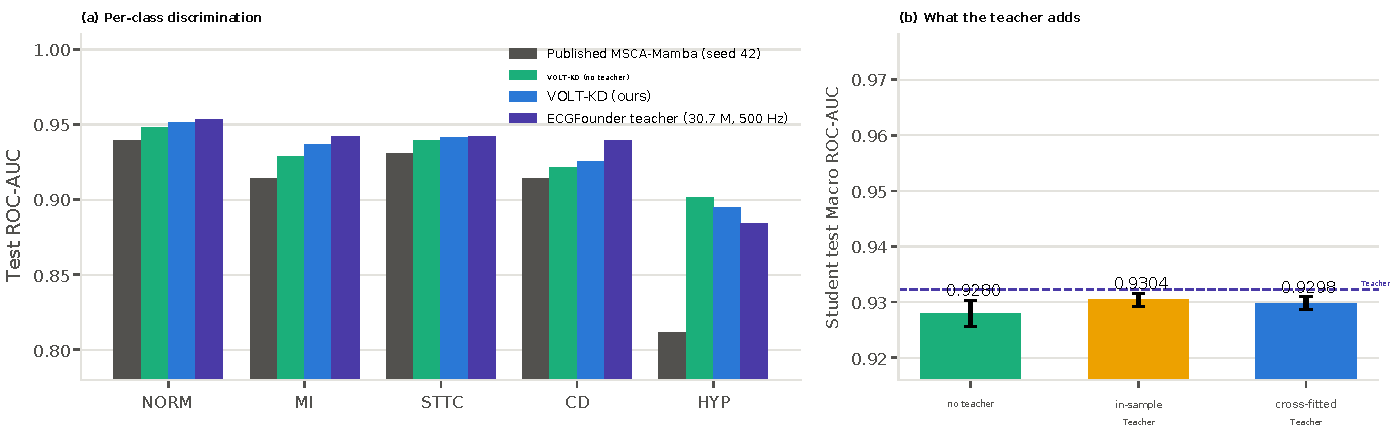
\includegraphics[width=\linewidth,height=0.38\textheight,keepaspectratio]{f24_teacher_student.pdf}
\caption{Classwise and aggregate results for ECGFounder teachers and VOLT-KD students. Teacher predictions average test logits from four held-out models; student results are five-seed means. The figure reports parameters per teacher, with ensemble totals in Table~\ref{tab:teacher}. Published MSCA-Mamba values use seed 42.}\label{fig:teacher}
\end{figure}


\subsection{Classwise and Subclass Analyses Locate Performance Gains}
Complete VOLT-KD improved overall classification while benefiting amplitude-related diagnoses (Figure~\ref{fig:perclass}). Five-seed ROC-AUC values were 0.9511, 0.9365, 0.9417, and 0.9251 for NORM, MI, STTC, and CD, respectively. HYP ROC-AUC was 0.8945, with AP 0.650. Discrimination across several classes within one compact backbone shows that millivolt inputs remain compatible with morphological and temporal representations. Lower HYP AP also reflects a more difficult precision--recall trade-off at low prevalence, making classwise evaluation essential for assessing amplitude preservation.
\begin{figure}[htbp]
\centering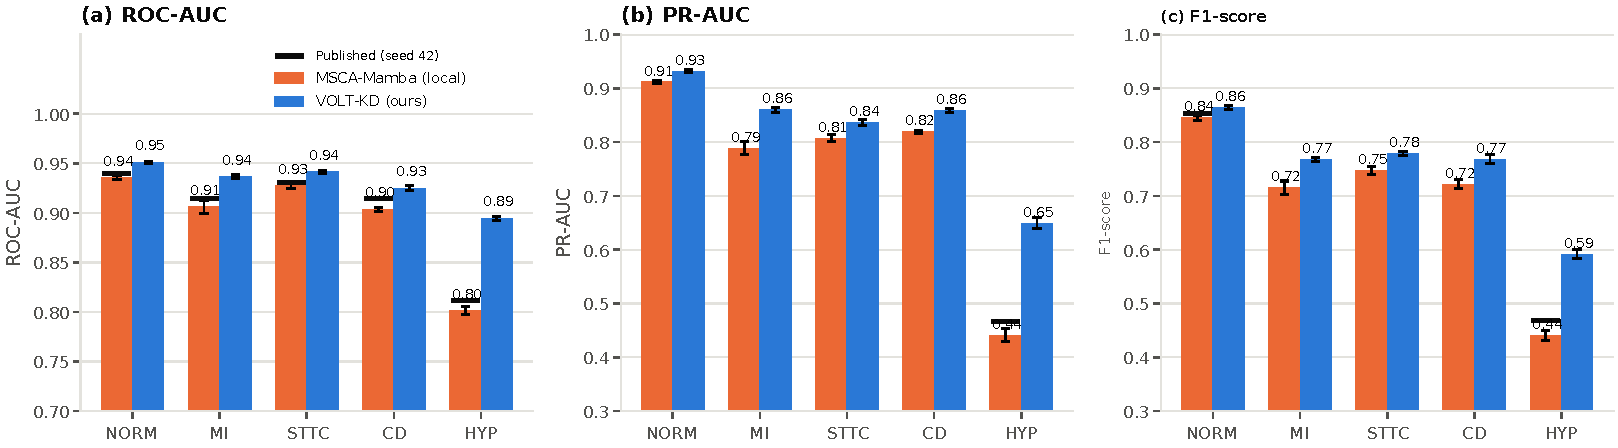
\includegraphics[width=\linewidth,height=0.38\textheight,keepaspectratio]{f07_per_class.pdf}
\caption{Classwise ROC-AUC, PR-AUC/AP, and F1 for complete VOLT-KD and local MSCA-Mamba. Bars and error bars indicate five-seed means and standard deviations. Black horizontal marks show the published MSCA-Mamba seed-42 results\cite{cetintas2026}.}\label{fig:perclass}
\end{figure}

For seed 42, VOLT-KD achieved HYP ROC-AUC 0.8930, AP 0.6607, and F1 0.6035, exceeding published MSCA-Mamba values of 0.8115, 0.4662, and 0.4682. Recall increased from 0.4924 to 0.6565. Across five seeds, complete VOLT-KD achieved HYP recall 0.6191 and specificity 0.9347 (Supplementary Table~S2). Better ranking in this amplitude-related class therefore accompanied detection of more positive recordings. Agreement between the literature comparison and fixed-backbone HYP input controls strengthens the link between voltage information and improved hypertrophy recognition.

Subclass evaluation further identified which diagnoses benefited from the input design (Figure~\ref{fig:subclass} and Supplementary Table~S4). Among LVH-labeled records, complete VOLT-KD predicted the parent HYP class as positive in 0.721 of cases, compared with 0.595 for local MSCA-Mamba. Parent-class detection rates increased by approximately 9.1 and 11.7 percentage points for IRBBB and AVB, respectively; AMI and IMI also improved. The LVH improvement agrees with the voltage probes and HYP input controls, connecting aggregate gains to a specific diagnosis with voltage-based criteria. The corresponding IVCD rate decreased from 0.327 to 0.289, showing that the shared backbone benefited different diagnostic morphologies unequally.
\begin{figure}[htbp]
\centering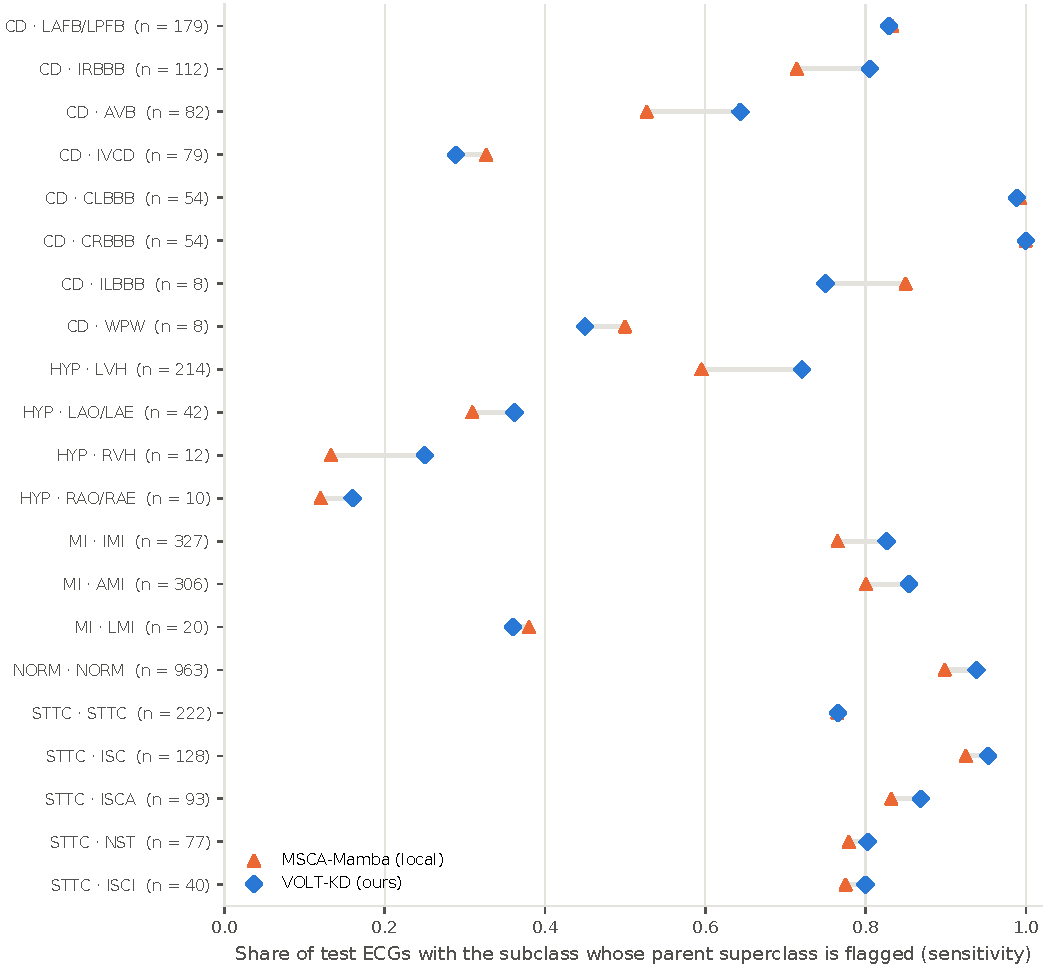
\includegraphics[width=\linewidth,height=0.58\textheight,keepaspectratio]{f16_subclass_sensitivity.pdf}
\caption{Parent-class detection rates for complete VOLT-KD and local MSCA-Mamba among records carrying each diagnostic subclass. Subclasses with at least five test recordings are included; values and sample sizes appear in Supplementary Table~S4.}\label{fig:subclass}
\end{figure}

\subsection{VOLT-KD Component Ablations and Student Simplification}
Input replacement, supervision removal, and structural simplification affected performance differently relative to complete VOLT-KD (Table~\ref{tab:loo} and Figure~\ref{fig:loo}). Variants changed the input to z-score, subclass losses, teacher-generation scheme, classification head, GRU layer, or network width, while retaining the corresponding remaining settings. These comparisons distinguish information preservation from network capacity and supervision targets.

Replacing millivolt inputs with z-score inputs reduced complete VOLT-KD's macro AUC from 0.9298 to 0.9179 and HYP AUC from 0.8945 to 0.8414. Retaining subclass and teacher supervision did not compensate for the loss of physical scale. Together with the superclass-only input gains, this result establishes amplitude preservation as a useful basis both before and within complete knowledge learning.
\begin{table}[htbp]
\centering\footnotesize
\setlength{\tabcolsep}{3pt}
\caption{Complete VOLT-KD and its component-ablation and structural-simplification variants. Values are means and standard deviations over the listed seed counts. Parameter counts refer to training.}\label{tab:loo}
\begin{tabularx}{\linewidth}{Yrrrrr}
\toprule
VOLT-KD student configuration & Seeds & Training parameters & Macro AUC & Macro F1 & HYP AUC \\
\midrule
VOLT-KD (complete, mV) & 5 & 112,364 & $0.9298\pm0.0012$ & $0.7542\pm0.0009$ & $0.8945\pm0.0018$ \\
VOLT-KD (z-score input) & 5 & 112,364 & $0.9179\pm0.0011$ & $0.7283\pm0.0022$ & $0.8414\pm0.0039$ \\
VOLT-KD (no subclass supervision) & 5 & 112,364 & $0.9299\pm0.0007$ & $0.7519\pm0.0031$ & $0.8943\pm0.0009$ \\
VOLT-KD (in-sample teacher) & 5 & 112,364 & $0.9304\pm0.0011$ & $0.7560\pm0.0047$ & $\boldsymbol{0.9001\pm0.0034}$ \\
VOLT-KD (noisy-OR head) & 3 & 111,239 & $\boldsymbol{0.9310\pm0.0004}$ & $0.7537\pm0.0023$ & $0.8970\pm0.0012$ \\
VOLT-KD (no GRU) & 3 & 59,692 & $0.9303\pm0.0003$ & $0.7541\pm0.0012$ & $0.8934\pm0.0031$ \\
VOLT-KD (half width) & 3 & \textbf{56,444} & $0.9298\pm0.0018$ & $\boldsymbol{0.7585\pm0.0029}$ & $0.8935\pm0.0024$ \\
\bottomrule
\end{tabularx}
\par\vspace{3pt}{\footnotesize All students use millivolt inputs except the z-score variant. Removing subclass supervision disables subclass hard-label and distillation losses but retains the auxiliary head, leaving training parameters unchanged. Complete VOLT-KD has 112,364 training parameters; the 107,189 in Table~\ref{tab:teacher} excludes the auxiliary head for deployment.}

\end{table}

Removing subclass supervision yielded macro AUC 0.9299, close to the complete model's 0.9298, while F1 decreased from 0.7542 to 0.7519. Subclass targets therefore contributed more to decisions than aggregate ranking. Half-width and no-GRU students used 56,444 and 59,692 training parameters, respectively, while achieving macro AUC 0.9298 and 0.9303. Comparisons paired on the three common seeds showed that simplified networks still formed effective representations from millivolt inputs. Amplitude preservation thus remained valuable without the full GRU or wider channels, providing evidence for further deployment compression.
\begin{figure}[htbp]
\centering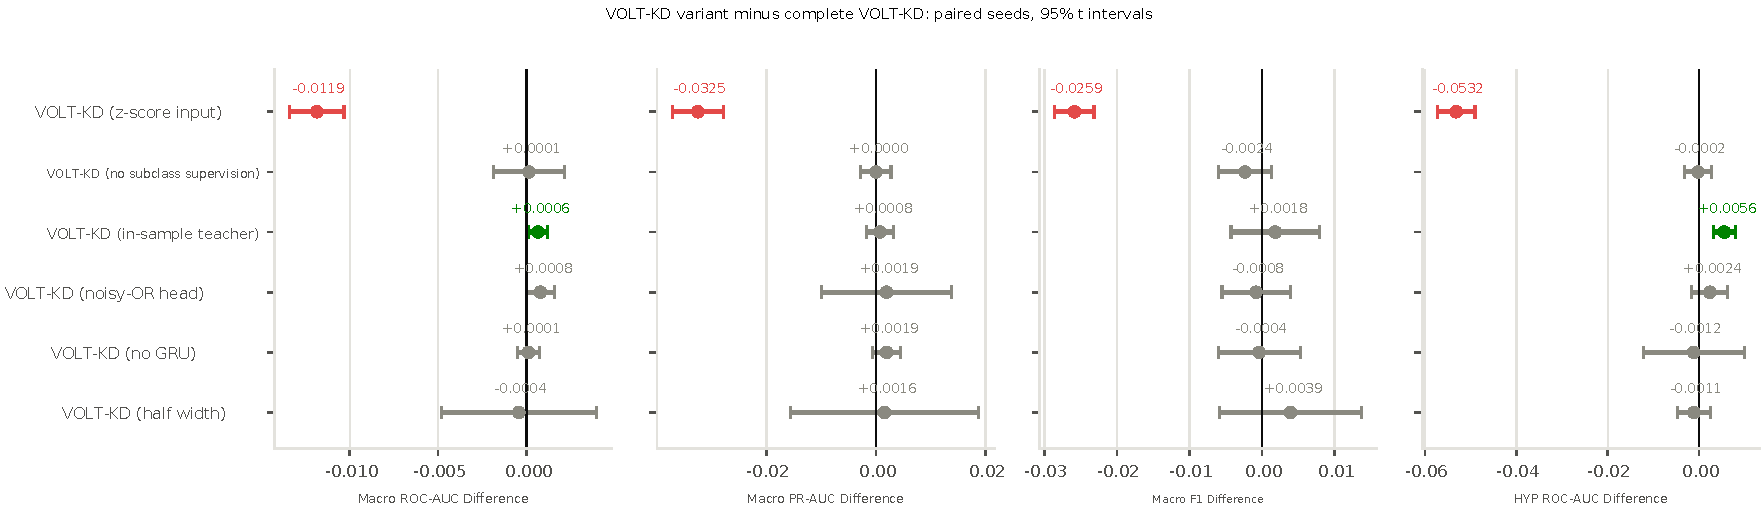
\includegraphics[width=\linewidth,height=0.45\textheight,keepaspectratio]{f12_ablation_leave_one_out.pdf}
\caption{Metric differences between VOLT-KD variants and complete VOLT-KD. Differences are variant minus complete model. Points and intervals use paired differences for identical seeds and 95\% $t$ intervals; configurations appear in Table~\ref{tab:loo}.}\label{fig:loo}
\end{figure}


\subsection{Gain and Lead Analyses Reveal Information Use}
VOLT-KD's HYP decisions changed systematically with input voltage gain (Figure~\ref{fig:gain}). Multiplying the same test recordings by 0.5, 1, and 2 yielded HYP-positive prediction rates of approximately 2.0\%, 13.3\%, and 52.3\%, respectively. Local MSCA-Mamba with per-lead standardization remained near 16.6\%. VOLT-KD's gain response shows that preserved voltage scale actively contributed to predictions instead of remaining unused input information.

Voltage probes link amplitude to hypertrophy labels, fixed-backbone controls show classification gains from retaining this information, and gain interventions confirm that model outputs respond to it. Together, these findings support incorporating physical voltage into compact representations. Gain sensitivity also makes acquisition units and device calibration relevant to output consistency. Preserving diagnostic amplitude therefore requires consistent conversion to millivolts during both training and use.
\begin{figure}[htbp]
\centering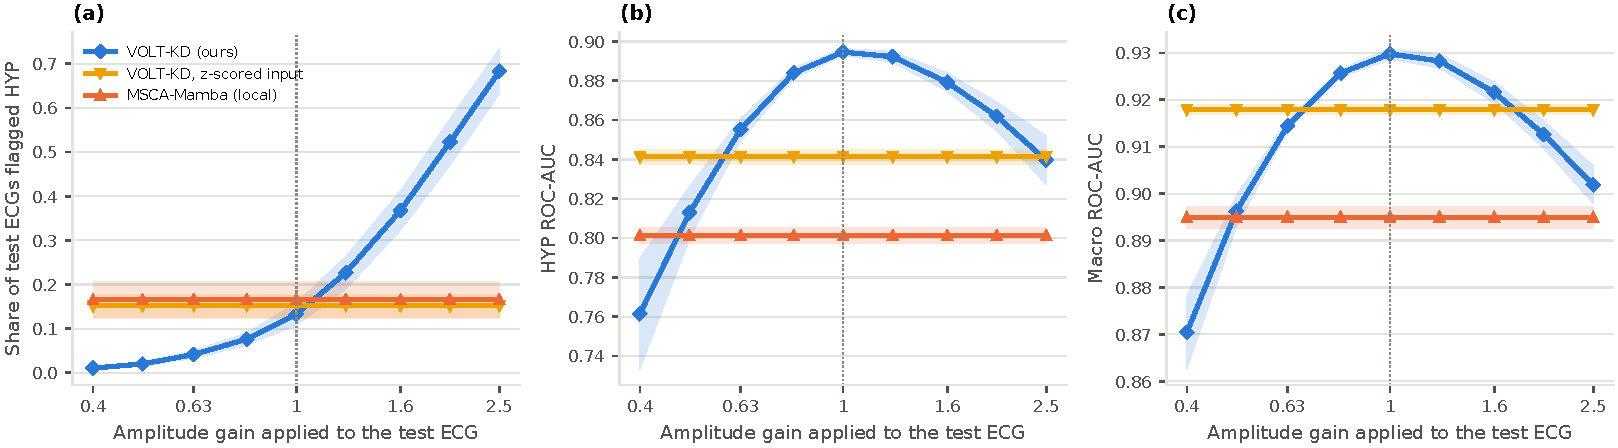
\includegraphics[width=\linewidth]{f13_gain_probe.pdf}
\caption{Responses of complete VOLT-KD, its z-score input control, and local MSCA-Mamba to global voltage gain. The same test waveforms are multiplied by each gain while model weights, labels, and validation-derived thresholds remain fixed.}
\label{fig:gain}
\end{figure}

Lead configurations alter the spatial observations available to the compact student. Table~\ref{tab:leads} compares complete twelve-lead VOLT-KD with separately trained six-limb-lead and lead-II students. All configurations share the backbone, millivolt preprocessing, and superclass, subclass, and twelve-lead teacher supervision. Unused channels are zeroed within the twelve-channel interface, allowing lead information to be assessed at fixed network capacity.

Six-limb-lead VOLT-KD achieved macro AUC $0.8964\pm0.0015$, exceeding the lead-II student's $0.8566\pm0.0010$ by 0.0398; HYP AUC values were 0.8476 and 0.7901, respectively. At fixed model size, additional limb leads supplied useful multidirectional electrical information. Complete twelve-lead VOLT-KD had the highest means across all four metrics, indicating that amplitude information and lead coverage jointly determine classification performance. A common backbone and training objective can serve different acquisition configurations. Compact computation provides the size advantage, while retaining more leads reduces information loss.

\begin{table}[htbp]
\centering\footnotesize
\setlength{\tabcolsep}{3pt}
\caption{Classification performance of complete twelve-lead VOLT-KD and separately trained six-limb-lead and lead-II students. Values are means and standard deviations over the listed seed counts; bold indicates the highest mean in each column.}\label{tab:leads}
\begin{tabularx}{\linewidth}{Yrrrrr}
\toprule
VOLT-KD student configuration & Seeds & Macro AUC & Macro AP & Macro F1 & HYP AUC \\
\midrule
VOLT-KD (twelve leads) & 5 & $\boldsymbol{0.9298\pm0.0012}$ & $\boldsymbol{0.8274\pm0.0020}$ & $\boldsymbol{0.7542\pm0.0009}$ & $\boldsymbol{0.8945\pm0.0018}$ \\
VOLT-KD (six limb leads) & 3 & $0.8964\pm0.0015$ & $0.7597\pm0.0036$ & $0.6922\pm0.0062$ & $0.8476\pm0.0003$ \\
VOLT-KD (lead II) & 3 & $0.8566\pm0.0010$ & $0.6828\pm0.0012$ & $0.6367\pm0.0008$ & $0.7901\pm0.0018$ \\
\bottomrule
\end{tabularx}
\par\vspace{3pt}{\footnotesize All students use twelve-lead ECGFounder soft labels, identical student structures, and the same supervision settings. Unused channels are zeroed in a twelve-channel input interface. Limb leads are I, II, III, aVR, aVL, and aVF; the single-lead variant retains only lead II.}

\end{table}
\subsection{Test-Subgroup Comparison of VOLT-KD and MSCA-Mamba}
Complete VOLT-KD's advantage over local MSCA-Mamba extended across multiple test subgroups (Figure~\ref{fig:subgroups} and Supplementary Table~S5). Fixed trained models were evaluated on the same PTB-XL test fold, grouped by sex, age, device, quality, and label co-occurrence. These comparisons test whether aggregate gains concentrate in a small subset of recording conditions.

For male and female groups, complete VOLT-KD achieved macro AUC 0.940 and 0.920, compared with 0.906 and 0.884 for local MSCA-Mamba. All four age groups improved; among patients aged 75 or older, AUC increased from 0.859 to 0.906. Gains across four major device groups were approximately 0.038--0.040. Improvements across population and device conditions indicate broad internal coverage rather than dominance by one high-performing subgroup.

Among 513 recordings flagged for noise, complete VOLT-KD achieved macro AUC 0.923, compared with 0.887 for local MSCA-Mamba. Among 508 recordings with multiple superclass labels, the corresponding values were 0.896 and 0.852. Gains under natural quality issues and coexisting abnormalities support the compact representation's ability to handle disturbed morphology and multiple diagnostic cues. These conditions extend the controlled input evaluation to within-subgroup performance of complete VOLT-KD. Absolute subgroup scores still differed, and the evidence remains bounded to PTB-XL's internal population and device distributions.
\begin{figure}[htbp]
\centering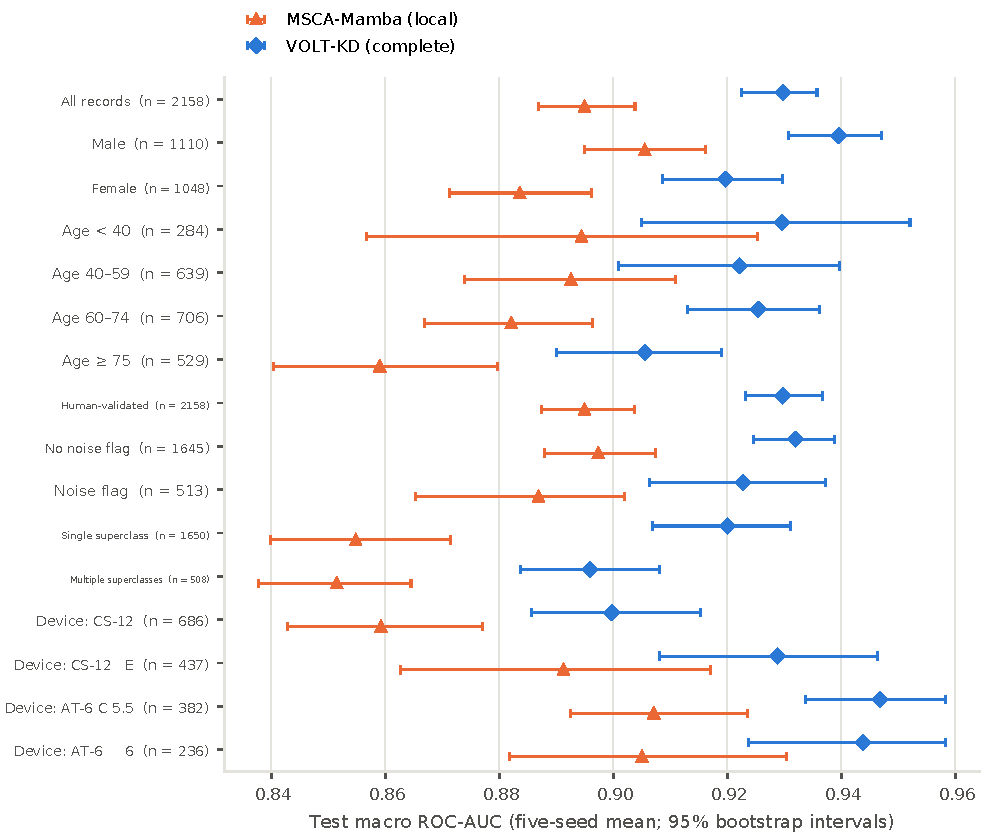
\includegraphics[width=\linewidth,height=0.57\textheight,keepaspectratio]{f17_subgroups.pdf}
\caption{Macro ROC-AUC of complete VOLT-KD and local MSCA-Mamba across test subgroups. Blue diamonds denote VOLT-KD and orange triangles local MSCA-Mamba. Points are five-seed mean metrics; horizontal bars are 95\% intervals from 300 within-subgroup recording-level bootstrap samples. Both models use the same test fold, grouped by demographic, device, quality, and label-co-occurrence conditions. Sample sizes and values appear in Supplementary Table~S5.}\label{fig:subgroups}
\end{figure}

\subsection{Probability Quality and Threshold-Based Decisions}
VOLT-KD also reduced error in the predicted probabilities (Table~\ref{tab:calib} and Figure~\ref{fig:calib}). Mean Brier score decreased from 0.096 for local MSCA-Mamba to 0.081 for complete VOLT-KD, with reductions in all five classes. HYP Brier score decreased from 0.088 to 0.067. Lower squared differences between probabilities and labels indicate improved overall probability quality beyond ranking alone. Mean expected calibration error (ECE) was approximately 0.037 for both models, with MI, CD, and HYP changing in the opposite direction to NORM and STTC. Reduced probability error and class-specific calibration improvements therefore represent distinct outcomes.
\begin{table}[htbp]
\centering\footnotesize
\caption{Classwise probability errors for complete VOLT-KD and local MSCA-Mamba. Values are five-seed means and standard deviations. Lower ECE and Brier scores are preferable.}\label{tab:calib}
\begin{tabularx}{\linewidth}{Yrrrr}
\toprule
Class & Local MSCA-Mamba ECE & VOLT-KD ECE & Local MSCA-Mamba Brier & VOLT-KD Brier \\
\midrule
NORM & $\boldsymbol{0.057\pm0.007}$ & $0.065\pm0.005$ & $0.106\pm0.002$ & $\boldsymbol{0.096\pm0.001}$ \\
MI & $0.039\pm0.005$ & $\boldsymbol{0.036\pm0.007}$ & $0.105\pm0.003$ & $\boldsymbol{0.086\pm0.002}$ \\
STTC & $\boldsymbol{0.022\pm0.002}$ & $0.027\pm0.004$ & $0.089\pm0.002$ & $\boldsymbol{0.079\pm0.002}$ \\
CD & $0.040\pm0.007$ & $\boldsymbol{0.034\pm0.001}$ & $0.091\pm0.001$ & $\boldsymbol{0.076\pm0.001}$ \\
HYP & $0.029\pm0.005$ & $\boldsymbol{0.022\pm0.005}$ & $0.088\pm0.001$ & $\boldsymbol{0.067\pm0.001}$ \\
\bottomrule
\end{tabularx}
\par\vspace{3pt}{\footnotesize ECE uses ten equal-width probability bins.}
\end{table}

\begin{figure}[htbp]
\centering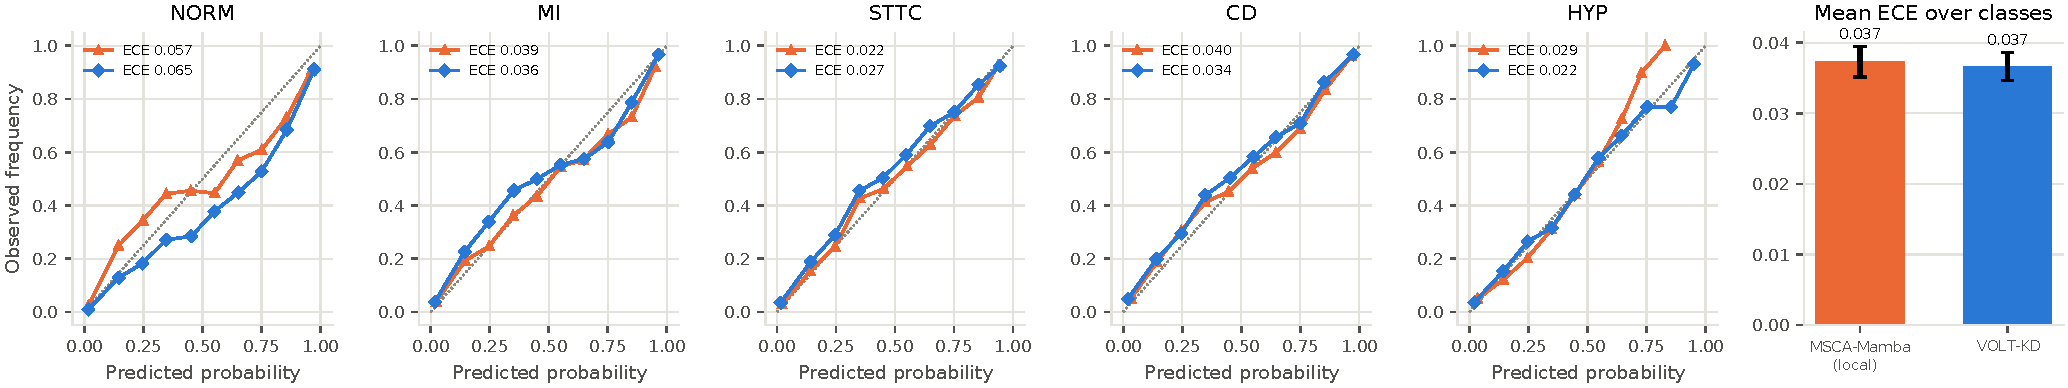
\includegraphics[width=\linewidth,height=0.50\textheight,keepaspectratio]{f19_calibration.pdf}
\caption{Classwise reliability curves and ECE for complete VOLT-KD and local MSCA-Mamba. Reliability curves compare predicted probabilities with observed positive frequencies.}\label{fig:calib}
\end{figure}

Decision curves assess threshold choices under different false-positive costs (Figure~\ref{fig:dca}). Net benefit is $\mathrm{NB}(t)=\mathrm{TP}/N-\mathrm{FP}/N\cdot t/(1-t)$. A threshold grid from 0.02 to 0.80 in steps of 0.02 yields 200 class--threshold combinations across five classes. VOLT-KD achieved net benefit no lower than local MSCA-Mamba in 195 combinations, or 97.5\%. This consistency indicates that the complete method's decision benefit extends across different false-positive weights rather than depending on a single operating point. Outcomes are database diagnostic labels, so the analysis supports algorithmic threshold decisions.
\begin{figure}[htbp]
\centering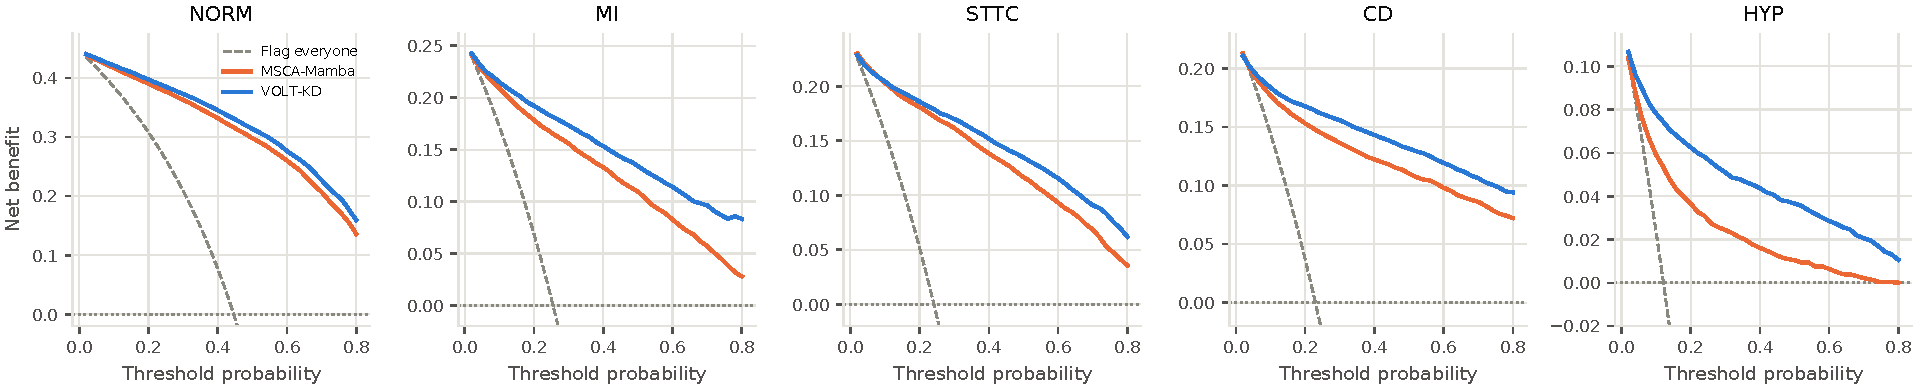
\includegraphics[width=\linewidth,height=0.40\textheight,keepaspectratio]{f20_decision_curves.pdf}
\caption{Decision curves for complete VOLT-KD and local MSCA-Mamba across five classes. Net benefit is averaged over five seeds. Reference lines classify every record as positive or negative; the positive NORM event is the normal label.}\label{fig:dca}
\end{figure}

\subsection{Input Perturbations in VOLT-KD and MSCA-Mamba}
The value of retained amplitude also depends on performance under noisy inputs. Figure~\ref{fig:noise} compares complete VOLT-KD and local MSCA-Mamba under baseline wander, Gaussian noise, and random lead zeroing, with trained weights fixed. Perturbations are applied to the same physical test signals before each model's original preprocessing and inference pipeline. This design evaluates the complete classifier's response to degraded input quality.

Baseline-wander amplitudes ranged from 0 to 2 mV, Gaussian-noise standard deviations from 0 to 0.2 mV, and zeroed lead counts from 0 to 8. Each perturbation had six tested levels (Supplementary Table~S6). Random lead zeroing probes unexpected channel loss in twelve-lead-trained models; separately retrained models for specific lead sets appear in Table~\ref{tab:leads}.

At 0.5 mV baseline wander, complete VOLT-KD achieved macro AUC 0.9058, compared with 0.7309 for local MSCA-Mamba. Relative to clean inputs, the decreases were approximately 0.0240 and 0.1641, respectively. At Gaussian-noise standard deviation 0.1 mV, AUC values were 0.9236 and 0.8499; zeroing four random leads yielded 0.8823 and 0.8315. Complete VOLT-KD retained higher AUC at every tested intensity. Its advantage therefore extended to progressively stronger interference and missing observations. Combined amplitude inputs, compact feature extraction, and augmentation retained useful diagnostic cues under these conditions. Performance still decreased under stronger interference and greater lead loss, showing that physical information preservation and signal quality must be considered together.
\begin{figure}[htbp]
\centering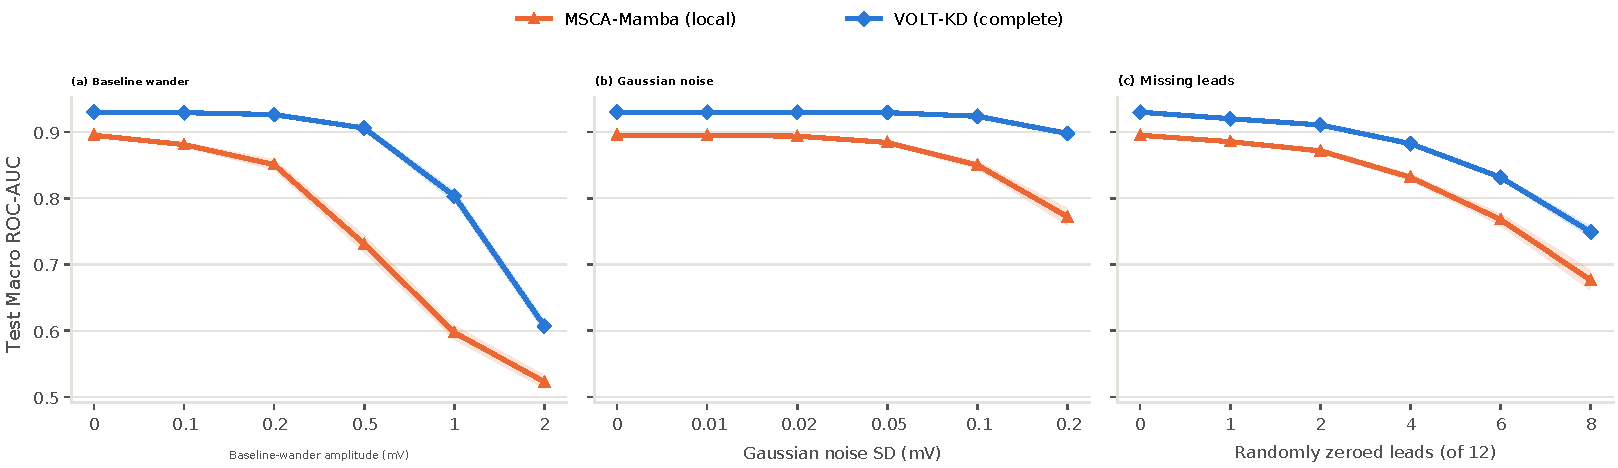
\includegraphics[width=\linewidth,height=0.43\textheight,keepaspectratio]{f18_noise_robustness.pdf}
\caption{Test macro ROC-AUC under input perturbations for complete VOLT-KD and local MSCA-Mamba. Blue diamonds denote VOLT-KD and orange triangles local MSCA-Mamba; points are five-seed means and shaded bands indicate $\pm1$ standard deviation. Panels show (a) low-frequency baseline wander, (b) Gaussian noise, and (c) random lead zeroing. Zero intensity denotes the original test inputs, and model weights are fixed. Complete values appear in Supplementary Table~S6.}\label{fig:noise}
\end{figure}


\subsection{Computational Benefits of the Compact Design}
VOLT-KD combined improved information use with lower computational cost (Table~\ref{tab:efficiency}). Relative to local MSCA-Mamba, deployed parameters decreased by 11.5\% and estimated computation by 81.6\%, with FP32 weights occupying 0.409 MiB. The larger reduction in computation than parameters agrees with reduced processing of long sequences. Multiscale depthwise convolution lowers temporal-filtering cost, shared pointwise projection controls channel mixing, and two downsampling stages reduce GRU sequence length to one quarter. The efficiency benefit therefore reflects both weight storage and the placement and sequence length of computation.

On the same NVIDIA GB10 platform, batch-256 throughput was 10,397 recordings/s for VOLT-KD and 3,199 for local MSCA-Mamba, a 3.25-fold increase. Single-thread CPU latency was 32.5 ms, approximately 0.33\% of the ten-second input duration. Lower arithmetic cost thus translated into higher batch-processing capacity, while the model also supported CPU inference. Single-record GPU latency was 1.68 ms versus 1.26 ms for the comparator, and peak GPU memory was 17.9 versus 5.8 MiB. The measured advantages were therefore strongest in batch throughput and parameter storage; deployment choices must also consider latency and memory requirements.

Achieving macro AUC 0.9298 with 107,189 deployed parameters shows that amplitude preservation and training-time knowledge learning do not require a high-capacity inference network. Parameter, computation, and throughput results jointly support the resource design: rich supervision during training and one compact path for physically scaled signals at inference.
\begin{table}[htbp]
\centering\footnotesize
\caption{Computational characteristics of eight architectures on the same NVIDIA GB10 platform. The VOLT-KD student's auxiliary head is removed. All parameter counts and computational measurements come from local implementations.}\label{tab:efficiency}
\begin{tabularx}{\linewidth}{Yrrrrrr}
\toprule
Model & Parameters & MFLOPs & \shortstack{GPU latency\\ms} & \shortstack{Throughput\\records/s} & \shortstack{GPU memory\\MiB} & \shortstack{CPU latency\\ms} \\
\midrule
VOLT-KD & 107,189 & \textbf{30.1} & 1.68 & 10,397 & 17.9 & 32.5 \\
MSCA-Mamba & 121,149 & 163.7 & 1.26 & 3,199 & 5.8 & -- \\
BiMamba & 214,077 & 292.7 & 1.66 & 1,788 & 6.6 & -- \\
Matched Conv1D & 120,435 & 169.0 & 1.05 & 7,506 & 2.4 & 6.0 \\
Matched GRU & 120,906 & 53.6 & 2.68 & 4,663 & 16.2 & 81.8 \\
Matched LSTM & 120,953 & 50.6 & 2.78 & 4,930 & 16.7 & 41.0 \\
Matched Transformer & 121,405 & 34.6 & 1.60 & 2,702 & 3.7 & 27.2 \\
Multiscale CNN & \textbf{51,141} & 34.6 & \textbf{0.54} & \textbf{17,066} & \textbf{1.5} & \textbf{1.9} \\
\bottomrule
\end{tabularx}
\par\vspace{3pt}{\footnotesize GPU latency uses batch size 1, throughput uses batch size 256, and CPU execution uses one thread. Parameter-matched controls and BiMamba are timed with untrained weights to measure architectural cost. MSCA-Mamba and the student use trained weights; -- indicates unavailable CPU timing.}
\end{table}


Among eight local architectures, VOLT-KD had the lowest estimated computation at 30.1 MFLOPs. Its batch throughput exceeded matched Conv1D, GRU, LSTM, Transformer, and both Mamba configurations, while the smaller multiscale CNN was faster (Figure~\ref{fig:efficiency}). These differences show that parameters, arithmetic operations, and measured speed respond differently to architectural organization. VOLT-KD combines strong classification performance with low computation, rather than minimizing every resource metric simultaneously.
\begin{figure}[htbp]
\centering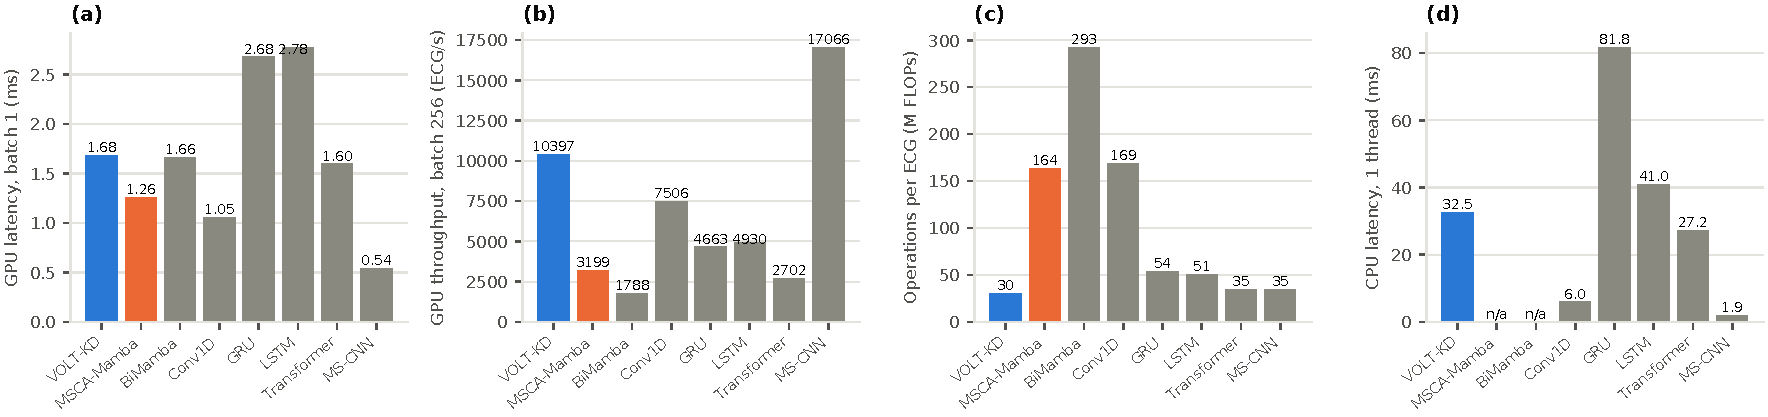
\includegraphics[width=\linewidth,height=0.45\textheight,keepaspectratio]{f15_efficiency.pdf}
\caption{Single-record GPU latency, batch throughput, estimated computation, and single-thread CPU latency for eight architectures on the same platform. Configurations and measurement units are provided in Table~\ref{tab:efficiency}.}\label{fig:efficiency}
\end{figure}

\section{Discussion}
The effective capacity of a lightweight ECG classifier depends on both network size and the diagnostic information remaining after preprocessing. Whereas MSCA-Mamba emphasizes multiscale feature extraction and temporal aggregation\cite{cetintas2026}, this study incorporates amplitude handling into the same design process. Voltage probes, input controls in two backbones, and gain interventions form a connected evidence chain. Millivolt representations retain hypertrophy-related voltage statistics, compact networks exploit those signals, and the retained amplitude influences predictions. Building on prior amplitude-processing research\cite{nolin2026}, we quantify the benefit and its class distribution in a classifier with approximately one hundred thousand parameters. This establishes the practical value of preserving input information for resource-constrained learning.

Input design, structural compression, and knowledge learning serve distinct roles in VOLT-KD. Amplitude preservation produces the main ranking gains, depthwise separable convolution and sequence downsampling reduces computation, and teacher probabilities improve macro F1 without changing student size. No-GRU and half-width variants retain high AUC, showing that strong performance does not require more complex temporal modules. Small teacher--student AUC differences alongside large parameter-count differences illustrate the separation of training supervision from deployment capacity. The HYP degradation under distillation nevertheless requires knowledge transfer to account for class-specific student strengths. Class-dependent distillation weights and millivolt-input teachers provide direct ways to investigate this trade-off.

Internal subgroup, perturbation, and reduced-lead analyses tested the design under different observation conditions. Complete-model gains extended across multiple populations and devices within the test set and persisted over the tested noise ranges. Reduced-lead training showed that a common backbone can accommodate different observation sets, although fewer leads reduce available diagnostic information. Amplitude sensitivity also requires consistent acquisition gains and millivolt conversion. Current conclusions concern short PTB-XL recordings and ECG interpretation labels; external datasets and real acquisition devices are needed to assess transfer across sources. Input comparisons jointly change centering, scaling, and associated augmentation, while teacher schemes differ in fine-tuning sample quantity. Factorial preprocessing experiments and teachers matched for fine-tuning data could further separate these effects.

\section{Conclusion}
We proposed VOLT-KD, combining millivolt inputs, compact multiscale representations, and hierarchical training-time knowledge learning for lightweight multi-label ECG classification. Voltage probes and controls in two backbones identified amplitude preservation as the main source of classification gains, particularly for hypertrophy-related labels. The complete model achieved macro ROC-AUC 0.9298 with 107,189 deployed parameters. Teacher supervision further improved macro F1 while revealing a measurable class-specific trade-off. Computational evaluation showed lower estimated operations and higher batch throughput. These findings support designing lightweight ECG classifiers around preserved diagnostic information, targeted training supervision, and compact inference.

\section*{Data Availability}
PTB-XL 1.0.3 is available through PhysioNet at \url{https://physionet.org/content/ptb-xl/1.0.3/}. Per-seed results, statistical summaries, and configuration records used in this study are retained by the research project.

\begingroup
\setlength{\bibsep}{3pt}
\begin{thebibliography}{99}
\bibitem{wagner2020} Wagner P, Strodthoff N, Bousseljot RD, et al. PTB-XL, a large publicly available electrocardiography dataset. \emph{Scientific Data}. 2020;7:154. \url{https://doi.org/10.1038/s41597-020-0495-6}.

\bibitem{cetintas2026} Cetintas D. MSCA-Mamba: A Compact Multi-Scale Mamba Network for Multi-Label ECG Classification. \emph{Diagnostics}. 2026;16(19):3135. Published 26 September 2026. \url{https://doi.org/10.3390/diagnostics16193135}.

\bibitem{behrouz2024} Behrouz A, Santacatterina M, Zabih R. Chimera: Effectively Modeling Multivariate Time Series with 2-Dimensional State Space Models. \emph{Advances in Neural Information Processing Systems}. 2024;37:119886--119918. \url{https://proceedings.neurips.cc/paper_files/paper/2024/hash/d8e80772c27beff4ae1676fb147bbf26-Abstract-Conference.html}.

\bibitem{feng2025} Feng N, Chen C, Du P, Gong C, Pei J, Huang D. MS-LTCAF: A Multi-Scale Lead-Temporal Co-Attention Framework for ECG Arrhythmia Detection. \emph{Bioengineering}. 2025;12(9):1007. \url{https://doi.org/10.3390/bioengineering12091007}.

\bibitem{luo2025} Luo K, Huang L, He H, Chen Y, You L, Chen S, Chen J, Liu C. Efficient and Interpretable ECG Abnormality Detection via a Lightweight DSCR-BiGRU-Attention Network with Demographic Fusion. \emph{Mathematics}. 2025;13(23):3882. \url{https://doi.org/10.3390/math13233882}.

\bibitem{malik2026} Malik A, Aras S. A lightweight hybrid framework integrating convolutional neural networks and fast Fourier transform for reliable and calibrated ECG-based cardiac abnormality detection. \emph{PLOS One}. 2026;21(7):e0354834. \url{https://doi.org/10.1371/journal.pone.0354834}.

\bibitem{sokolow1949} Sokolow M, Lyon TP. The ventricular complex in left ventricular hypertrophy as obtained by unipolar precordial and limb leads. \emph{American Heart Journal}. 1949;37(2):161--186. \url{https://doi.org/10.1016/0002-8703(49)90562-1}.

\bibitem{casale1985} Casale PN, Devereux RB, Kligfield P, et al. Electrocardiographic detection of left ventricular hypertrophy: development and prospective validation of improved criteria. \emph{Journal of the American College of Cardiology}. 1985;6(3):572--580. \url{https://doi.org/10.1016/S0735-1097(85)80115-7}.

\bibitem{hancock2009} Hancock EW, Deal BJ, Mirvis DM, et al. AHA/ACCF/HRS Recommendations for the Standardization and Interpretation of the Electrocardiogram: Part V: Electrocardiogram Changes Associated With Cardiac Chamber Hypertrophy. \emph{Journal of the American College of Cardiology}. 2009;53(11):992--1002. \url{https://doi.org/10.1016/j.jacc.2008.12.015}.

\bibitem{nolin2026} Nolin-Lapalme A, Sowa A, Delfrate J, et al. Foundation models for electrocardiogram interpretation: clinical implications. \emph{European Heart Journal}. 2026;47(18):2174--2186. \url{https://doi.org/10.1093/eurheartj/ehaf1119}.

\bibitem{li2025} Li J, Aguirre AD, Moura V, et al. An Electrocardiogram Foundation Model Built on over 10 Million Recordings. \emph{NEJM AI}. 2025;2(7). \url{https://doi.org/10.1056/AIoa2401033}.

\bibitem{mckeen2025} McKeen K, Masood S, Toma A, Rubin B, Wang B. ECG-FM: an open electrocardiogram foundation model. \emph{JAMIA Open}. 2025;8(5):ooaf122. \url{https://doi.org/10.1093/jamiaopen/ooaf122}.

\bibitem{qin2023} Qin Y, Sun L, Chen H, Yang W, Zhang WQ, Fei J, Wang G. MVKT-ECG: Efficient single-lead ECG classification for multi-label arrhythmia by multi-view knowledge transferring. \emph{Computers in Biology and Medicine}. 2023;166:107503. \url{https://doi.org/10.1016/j.compbiomed.2023.107503}.

\bibitem{mehari2022} Mehari T, Strodthoff N. Self-supervised representation learning from 12-lead ECG data. \emph{Computers in Biology and Medicine}. 2022;141:105114. \url{https://doi.org/10.1016/j.compbiomed.2021.105114}.

\bibitem{vaid2023} Vaid A, Jiang J, Sawant A, et al. A foundational vision transformer improves diagnostic performance for electrocardiograms. \emph{npj Digital Medicine}. 2023;6:108. \url{https://doi.org/10.1038/s41746-023-00840-9}.

\bibitem{mert2026} Mert YE, Akdo\u{g}an E, \"{U}vet H. Multi-Label 12-Lead ECG Classification on the PTB-XL Dataset: A Comparative Evaluation of Deep Learning Architectures and Heterogeneous Ensemble Approaches. \emph{arXiv preprint}. 2026;arXiv:2609.12803. Posted 11 September 2026. \url{https://arxiv.org/abs/2609.12803}.

\bibitem{howard2017} Howard AG, Zhu M, Chen B, et al. MobileNets: Efficient Convolutional Neural Networks for Mobile Vision Applications. \emph{arXiv}. 2017;1704.04861. \url{https://arxiv.org/abs/1704.04861}.

\bibitem{cho2014} Cho K, van Merrienboer B, Gulcehre C, et al. Learning Phrase Representations using RNN Encoder--Decoder for Statistical Machine Translation. \emph{Proceedings of EMNLP}. 2014;1724--1734. \url{https://doi.org/10.3115/v1/D14-1179}.

\bibitem{hinton2015} Hinton G, Vinyals O, Dean J. Distilling the Knowledge in a Neural Network. \emph{arXiv}. 2015;1503.02531. \url{https://arxiv.org/abs/1503.02531}.

\bibitem{loshchilov2019} Loshchilov I, Hutter F. Decoupled Weight Decay Regularization. \emph{International Conference on Learning Representations}. 2019. \url{https://openreview.net/forum?id=Bkg6RiCqY7}.
\bibitem{jiang2025} Jiang H, Mutahira H, Wei S, Muhammad MS. ECG-Mamba: Cardiac Abnormality Classification With Non-Uniform-Mix Augmentation on 12-Lead ECGs. \emph{IEEE Journal of Translational Engineering in Health and Medicine}. 2025;13:461--470. \url{https://doi.org/10.1109/JTEHM.2025.3613609}.

\bibitem{luomar2026} Luo K, He H, Chen Y, et al. MAR-GCNet: Multi-label abnormal detection of electrocardiograms by combining multiscale features and graph convolutional networks. \emph{Biomedical Signal Processing and Control}. 2026;119:109841. \url{https://doi.org/10.1016/j.bspc.2026.109841}.

\bibitem{weimann2025} Weimann K, Conrad TOF. Self-supervised pre-training with joint-embedding predictive architecture boosts ECG classification performance. \emph{Computers in Biology and Medicine}. 2025;196:110809. \url{https://doi.org/10.1016/j.compbiomed.2025.110809}.

\bibitem{lin2026} Lin S, Li Z, Wu Q, Chen Y, Yang Y, Zhao H. A self-supervised electrocardiogram foundation model for empowering cardiovascular disease prediction and genetic factor discovery. \emph{Nature Communications}. 2026;17:5771. \url{https://doi.org/10.1038/s41467-026-72436-2}.

\bibitem{khattak2026} Khattak GR, Patlatzoglou K, Barker J, et al. Data distribution impacts the performance and generalisability of contrastive learning-based foundation models of electrocardiograms. \emph{PLOS Digital Health}. 2026;5(9):e0001623. \url{https://doi.org/10.1371/journal.pdig.0001623}.

\bibitem{beigzadeh2026} Beigzadeh N, Fathi A. HMT-KD: Lightweight deep learning model for ECG analysis using hierarchical multi-teacher knowledge distillation framework. \emph{Applied Soft Computing}. 2026;196:115038. \url{https://doi.org/10.1016/j.asoc.2026.115038}.

\bibitem{qian2026} Qian C, Sun Z, Wang C, Tian E, Hu X. Self-knowledge distillation from attention-enhanced multi-branch residual network for 12-lead electrocardiogram arrhythmia classification. \emph{Digital Signal Processing}. 2026;176:106043. \url{https://doi.org/10.1016/j.dsp.2026.106043}.

\bibitem{yisimitila2025} Yisimitila T, Wang C, Hou M, et al. Bridging clinical knowledge and AI: an interpretable transformer framework for ECG diagnosis. \emph{npj Digital Medicine}. 2025;9:41. Published online 19 December 2025. \url{https://doi.org/10.1038/s41746-025-02215-8}.

\bibitem{nguyen2025} Nguyen HD, Pham TT, Le N, Nguyen V. TolerantECG: A Foundation Model for Imperfect Electrocardiogram. \emph{Proceedings of the 33rd ACM International Conference on Multimedia}. 2025;8097--8105. \url{https://doi.org/10.1145/3746027.3755287}.

\bibitem{su2026} Su H, Wang S, Wang H, Qiu K. An Edge--Cloud Collaborative ECG-Assisted Diagnostic System Leveraging Cross-Lead Knowledge Distillation and Large Language Models. \emph{Sensors}. 2026;26(12):3753. \url{https://doi.org/10.3390/s26123753}.
\end{thebibliography}
\endgroup
\end{document}
